\documentclass[11pt,]{article}
\usepackage[left=1in,top=1in,right=1in,bottom=1in]{geometry}
\newcommand*{\authorfont}{\fontfamily{phv}\selectfont}
\usepackage[]{mathpazo}


  \usepackage[T1]{fontenc}
  \usepackage[utf8]{inputenc}



\usepackage{abstract}
\renewcommand{\abstractname}{}    % clear the title
\renewcommand{\absnamepos}{empty} % originally center

\renewenvironment{abstract}
 {{%
    \setlength{\leftmargin}{0mm}
    \setlength{\rightmargin}{\leftmargin}%
  }%
  \relax}
 {\endlist}

\makeatletter
\def\@maketitle{%
  \newpage
%  \null
%  \vskip 2em%
%  \begin{center}%
  \let \footnote \thanks
    {\fontsize{18}{20}\selectfont\raggedright  \setlength{\parindent}{0pt} \@title \par}%
}
%\fi
\makeatother




\setcounter{secnumdepth}{3}


\usepackage{graphicx,grffile}
\makeatletter
\def\maxwidth{\ifdim\Gin@nat@width>\linewidth\linewidth\else\Gin@nat@width\fi}
\def\maxheight{\ifdim\Gin@nat@height>\textheight\textheight\else\Gin@nat@height\fi}
\makeatother
% Scale images if necessary, so that they will not overflow the page
% margins by default, and it is still possible to overwrite the defaults
% using explicit options in \includegraphics[width, height, ...]{}
\setkeys{Gin}{width=\maxwidth,height=\maxheight,keepaspectratio}

\title{Análisis de la Familia de Moraceae en una Parcela de 50 Hectáreas,
Dentro de la Isla Barro Colorado  }



\author{\Large José Abreu Díaz\vspace{0.05in} \newline\normalsize\emph{Estudiante de geografía, Universidad Autónoma de Santo Domingo (UASD)}  }


\date{}

\usepackage{titlesec}

\titleformat*{\section}{\normalsize\bfseries}
\titleformat*{\subsection}{\normalsize\itshape}
\titleformat*{\subsubsection}{\normalsize\itshape}
\titleformat*{\paragraph}{\normalsize\itshape}
\titleformat*{\subparagraph}{\normalsize\itshape}

\titlespacing{\section}
{0pt}{36pt}{0pt}
\titlespacing{\subsection}
{0pt}{36pt}{0pt}
\titlespacing{\subsubsection}
{0pt}{36pt}{0pt}





\newtheorem{hypothesis}{Hypothesis}
\usepackage{setspace}

\makeatletter
\@ifpackageloaded{hyperref}{}{%
\ifxetex
  \PassOptionsToPackage{hyphens}{url}\usepackage[setpagesize=false, % page size defined by xetex
              unicode=false, % unicode breaks when used with xetex
              xetex]{hyperref}
\else
  \PassOptionsToPackage{hyphens}{url}\usepackage[unicode=true]{hyperref}
\fi
}

\@ifpackageloaded{color}{
    \PassOptionsToPackage{usenames,dvipsnames}{color}
}{%
    \usepackage[usenames,dvipsnames]{color}
}
\makeatother
\hypersetup{breaklinks=true,
            bookmarks=true,
            pdfauthor={José Abreu Díaz (Estudiante de geografía, Universidad Autónoma de Santo Domingo (UASD))},
             pdfkeywords = {Isla Barro Colorado, PH, varaible ambiental numérica, variable ambiental
nominal, Moraceae, pendiente, abundancia global, riqueza global, Canal
de Panamá.},  
            pdftitle={Análisis de la Familia de Moraceae en una Parcela de 50 Hectáreas,
Dentro de la Isla Barro Colorado},
            colorlinks=true,
            citecolor=blue,
            urlcolor=blue,
            linkcolor=magenta,
            pdfborder={0 0 0}}
\urlstyle{same}  % don't use monospace font for urls

% set default figure placement to htbp
\makeatletter
\def\fps@figure{htbp}
\makeatother

\usepackage{pdflscape} \newcommand{\blandscape}{\begin{landscape}}
\newcommand{\elandscape}{\end{landscape}} \usepackage{float}
\floatplacement{figure}{H}
\newcommand{\beginsupplement}{ \setcounter{table}{0} \renewcommand{\thetable}{S\arabic{table}} \setcounter{figure}{0} \renewcommand{\thefigure}{S\arabic{figure}} }


% add tightlist ----------
\providecommand{\tightlist}{%
\setlength{\itemsep}{0pt}\setlength{\parskip}{0pt}}

\begin{document}
	
% \pagenumbering{arabic}% resets `page` counter to 1 
%
% \maketitle

{% \usefont{T1}{pnc}{m}{n}
\setlength{\parindent}{0pt}
\thispagestyle{plain}
{\fontsize{18}{20}\selectfont\raggedright 
\maketitle  % title \par  

}

{
   \vskip 13.5pt\relax \normalsize\fontsize{11}{12} 
\textbf{\authorfont José Abreu Díaz} \hskip 15pt \emph{\small Estudiante de geografía, Universidad Autónoma de Santo Domingo (UASD)}   

}

}








\begin{abstract}

    \hbox{\vrule height .2pt width 39.14pc}

    \vskip 8.5pt % \small 

\noindent El presente artículo, está basado en el análisis de Moraceae existentes
en la Isla de Barro Colorado,para el mismo se emplean mapas y tablas con
muestras en un parcela de 50 ha, dividida en celdas de una ha cada una.
Empleando un estudio multimodal, se destacan las variables propuestas
como son medidas de PH, abundancia global, abundancia específica
(familia), riqueza global, riqueza específica, mapa de pendientes, y los
cuadros de variables ambientales numéricas. En todas ellas se aprecia un
crecimiento exponencial de la familia bajo estudio. Con el objetivo de
enteder la razón de existencia de las condiciones que han dado origen a
la amplia riqueza y abundancia de BCI, en el caso de la familia bajo
estudio, resalto el contexto político e histórico en que ha surgido la
isla, y su situación geográfica. Dejando claro que pudieran existir
otros grandes laboratorios de alcance global, aunque claro, no con la
misma posición grográfica estratégica que tiene esta isla en el Istmo de
Panamá


\vskip 8.5pt \noindent \emph{Keywords}: Isla Barro Colorado, PH, varaible ambiental numérica, variable ambiental
nominal, Moraceae, pendiente, abundancia global, riqueza global, Canal
de Panamá. \par

    \hbox{\vrule height .2pt width 39.14pc}



\end{abstract}


\vskip 6.5pt


\noindent  \section{Introducción}\label{introducciuxf3n}

Así como puede estar integrada una familia convencional, también las
familias de plantas presentan unos criterios de agrupación que hacen de
cada grupo botánico, verdaderas unidades identificables (Van Devender et
al., 2010). Los senderos a seguir nos podrían encaminar por un sinfín de
rutas alternativas, según, Van Devender et al. (2010), la flora del
estado de Sonora con un área de 184934 km2, actualmente tiene 3652
taxones específicos e intraespecíficos en 188 familias y 1103 géneros.
La organización de las plantas en familias constituye una respuesta
específica al orden en que la ecología, como ciencia que estudia las
categorías agrupacionales que presentan los organismos en sus
interacciones, ordena las unidades de grupos de plantas. Viendo que la
ecología es la forma sistemática de estudiar las diversas dimensiones
que resultan de la interacción entre organismos diversos, nos apoyamos
en la biogeografía, con la intención de conocer los emplazamientos que
ocupan esos grupos de organismos, especialmente de plantas. En este
manuscrito se pretenden entender los aspectos fundamentales de la
familia de plantas conocida como Moraceae, partiendo del estudio de
gráficos, tablas y diagramas procedentes de invstigaciones realizadas en
la Isla Barro Colorado, en Panamá. Según, Clement \& Weiblen (2009), la
familia Moracea comprende 37 géneros y aproximadamente 1100 especies en
regiones tropicales y templadas en todo el mundo. En América se aprecia
una amplia dsitribución de las especies de esta familia, como lo es en
el territorio de México, en las zonas de Sinaloa, o Chiapas, siendo de
gran importancia para la comunidad de frugivoros que se alimentan de las
mismas. Entre las especies reconocidas, se destacan: Brosimun
alicastrum, Maclura tinctoria, Ficus mexicana, Ficus petiolaris, Ficus
cotinifolia, Ficus spp. De esta misma distribución existen importantes
trabajos, como son: Magallanes, Rocha, \& Terán (n.d.), y
Piedra-Malagón, Ramírez Rodríguez, \& Ibarra -Manríquez (2006). En ese
orden pretendo identificar otras zonas del mundo donde podrían existir
ejemplares de estas plantas correspondientes a los tipos de especies, y
cuáles zonas presentan condiciones favorables para el predominio de las
mismas, partiendo del análisis de los trabajos realizados en Isla Barro
Colorado. En los últimos años pareciera que el papel de la geografía y
de la ecología se confinara más a un grupo de investigadores que hace su
trabajo más por vocación, que por farándula y fama, a sabiendas que
muchos estudiosos se han dedicado más a estar en los medios que en
centrarse en el trabajo para el cual se han formado que en este caso es
la investigación, no el entretenimiento. Hacer ciencia es asumir un
compromiso con la verdad, con la sociedad que espera respuestas serias
para tomar grandes decisiones, pero el amarillismo nos ha oxidado un
poco el compromiso con el deber. La ciencia después de la religión es
como el único puerto en el cual se pued anclar el raciocinio, por ende
debe ser depositaria dicha profesión de respeto y realización con
cordura, pero sobretodo de la mano del talento y el compromiso. A
sambiendas de que la Isla Barro Colorado no es un espacio en donde se
venga realizando ciencia de antaño, no existe allí, partiendo del
territorio, una culutra cintífica milenaria que conserve los grandes
hitos del quehacer intelectual, pero el pensamiento viaja de unas
sociedades a otras y en cada latitud aquiere matices que le hacen ser.
Sin embargo cada lugar para la ciencia resulta ser siempre nuevo y sobre
todo si se trata de un lugar interoceánico como lo es la Isla Barro
Colorado. Antes (siglos XVI, XVII, XVII Y XIX) el istmo de Panamá era
solo visto como una ruta transoceánica, y de hecho hoy ostenta al
legendario Canal homónimo como una arteria marítima que suple a la
economía a escala global. Pero además de ruta comercial es el
emplazamiento de BCI, escenario de este trabajo científico. Y que bueno
que se ha roto el paradigma de ser el antiguo Egipto, la tierra fértil
de la investigación, aunque evidentemente son campos de estudio
distintos, pero Latinoamérica en su quehacer histórico se ha dejado
colocar un estereotipo de aversión a la investigación. Como que somos
buenos para la transculturación y todo aquello que sea plástico, pero no
para incursionar en algo tan serio como lo es el hacer ciencia. Pero
seguimos creciendo, y es cierto que nos independizamos, y adquirimos
indentidad júridica, pero las costumbres y las mantalidades aún nos
abruman. Necesitamos independizar el talento, y darle soberanía al
genio, así manejaremos un terremoto o cualquier otro evento natural sin
que antes lo depuren los del norte.

\section{Metodología}\label{metodologuxeda}

Apoyándome en los trabajos realizados en la Isla de Barro Colorado,
mediante un anális inductivo, pretendo dilucidar los datos estadísticos
más pertinentes sobre la familia de plantas conocidas como Moraceae.
Dejando claro que en otras zonas del continente existen importantes
trabajos sobre esta familia de plantas, susceptibles de estudios debido
en gran parte al soporte que constituyen en la alimentación de una
amplia comunidad de frugívoros. Tomando como escenario esa pequeña isla
del istmo de Panamá, empleando un serie de recursos que han derivado de
profundas investigaciones, intento crear una nueva fisonomía a esta
familia de plantas, o por lo menos generar algo nuevo para quienes
consumen este tipo de artículos. La isla de Barro Colorado se formó tras
la creación del lago Gatún en 1913, durante la construcción del Canal de
Panamá (1904-1914), la isla de 15 kilómetros cuadrados, alberga una de
las estaciones más antiguas de investigación tropical del mundo donde se
han llevado a cabo estudios por más de 100 años.\\
La Isla Barro Colorado o BCI, por sus siglas en inglés, es uno de los
puntos geográficos más estudiados en el mundo, es como una especie de
Meca para los investigadores que quieren desarrollar allí sus estudios,
muchas veces acompañados de sus estudiantes, estudiantes que en lo
adelante también realizarán sus propias investigaciones por separado. En
dicha isla todo está registrado, cada comunidad de insectos, plantas y
otros animales, están debidamente mapeados, con inscripciones por
doquier. Tal vez por la Amplia diversidad de orgaismos que allí
predominana, se hace esta clase de inferencia en esta isla que se ha
convertido en un laboratorio global, y ese es el caso que me compete,
seguir ese pequeño trillo prar llegar a grandes verdades que requieren
de una cantidad de recursos unaudita y tiempo, por el momento no
disponibles si nos embarcaramos en hacer un itinerario parecido al de
Darwin o el de Humboldt. Algunos estudios como los de Fredericksen,
Justiniano, Rumiz, McDonald, \& Aguape (n.d.), resaltan la importancia
de las moraceae en el sentido de que sirven de alimentos a una amlpia
comunidad de frugivoros, pero los cierto es que también, tienen gran
importancia en el sector maderero. Como se dijo en un principio, todo el
material de apoyo, proviene de las investigaciones de la Isla de Barro
Colorado, el cual consiste en el empleo de tablas, cuadros, mapas, y
otros diagramas que proceden de sendas investigaciones. Para el estudio
de las variables ambientales se han empleado los cuadros de 1 Ha de BCI.
Variables ambientales numéricas escaladas de 0 a 1, para el estudio de
las pendientes, se emplea el mapa de curbas de nivel de la isla. También
se ha empleado el mapa que refleja el PH de este espacio insular.
También se establecen correlaciones a partir de estos recursos
científicos que son el fruto de largos proceos de estudio.

Este es el escenario de nuestro estudio, ver figura
\ref{fig:bci_map #1}.

\begin{figure}
\centering
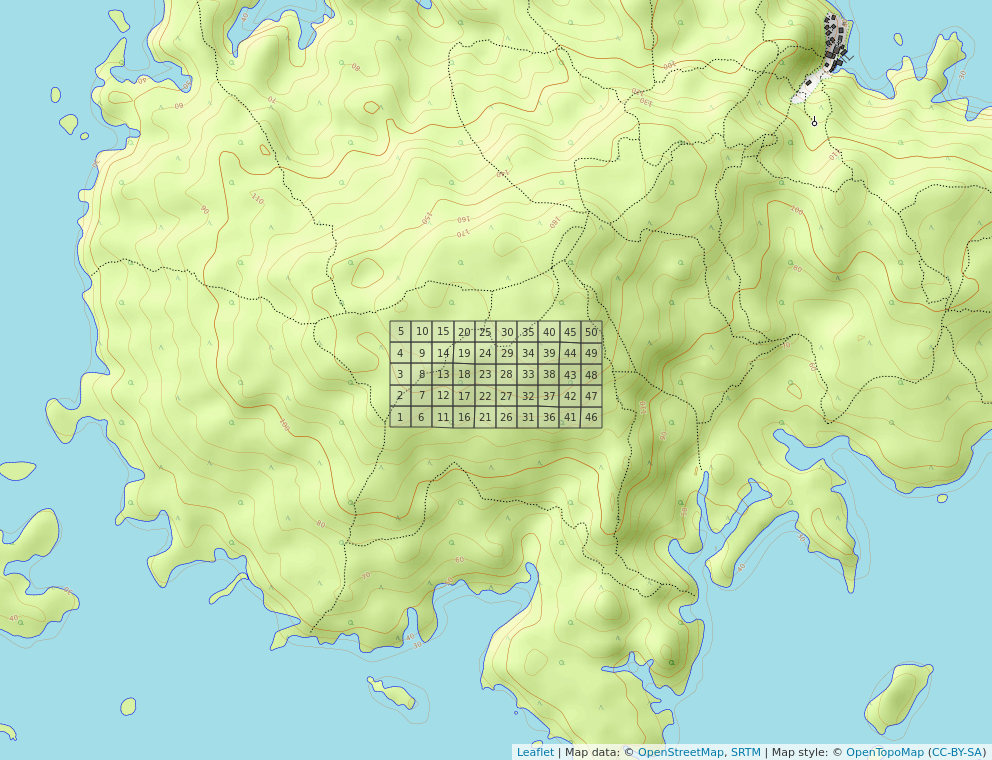
\includegraphics[width=1.00000\textwidth]{mapa_cuadros.png}
\caption{mapa de Isla Barro Colorado cuadros\label{fig:bci_map}}
\end{figure}

Por igual se emplean los cuadros de variables ambientales nominales de 1
Ha de BCI, constituida por categoría de edad, habitat, geología y
quebrada. Otro recurso de vital importancia son las variables
ambientales numéricas escaladas de 0 a 1 de una Ha de BCI. La
interacción con estas fuentes de información ayudan a tener una
aproximación más concreta sobre la diversidad con relación a la familia
que nos compete. Es cierto que el condicionamiento de diversas especies
de plantas en distintos espacios termina creando casos de escasa
homogeneidad, que de una u otra forma se rompa el patrón de similitud.
Es por ello que en este trabajo se maneja más un enfoque particular de
la realidad existente en BCI. Algunos estudios demuestran que las
moraceae no solo sireven de alimento a los frugivoros, o como soporte en
la industria maderera, también sirven de huesped a algunas especies como
es el caso de las avispas, las cuales se desarrollan en las flores
femeninas de dichas plantas según Cardona, De Ulloa, \& Kattan (2007).
Otros estudios abordan las propiedades químicas de dichas plantas, este
trabajo buca definir las características más notables de esta familia de
plantas apoyándonos en el escenario de BCI. Es notorio el mapa de
variables ambientales nominales. Los demás recursos se verán en la
medidad que se deasarrolla el trabajo, siguiendo el orden que en un
principio nos hemos propuesto.

\section{Resultados}\label{resultados}

A continuación se muestran las mediciones de PH, mapa de pendientes,
mapas de abundancia, tanto global como de la familia, mapa de riqueza
global y de la familia, variables ambientales numéricas, y nominales en
una parcela de 50 hectáreas, integrada por subdivisiones de una
hectárea, todo ello correspondiente a la familia de las Moraceae. En el
caso del PH tenemos que es ácido, sgún los mapas y diagramas
consultados, estas condiciones para las Moraceae, y cualquier otra
especie en condiciones extremas, sería perjudicial. El PH del suelo es
importante porque los vegetales solo pueden absorver a los minerales
disueltos y la variación del PH modifica el grado de solubilidad de los
minerales y nutrientes. En el siguiente mapa, se pueden apreciar las
medidas de PH presentes en la Isla Barro Colorado en una parcela de 50
hectáreas:

\begin{figure}
\centering
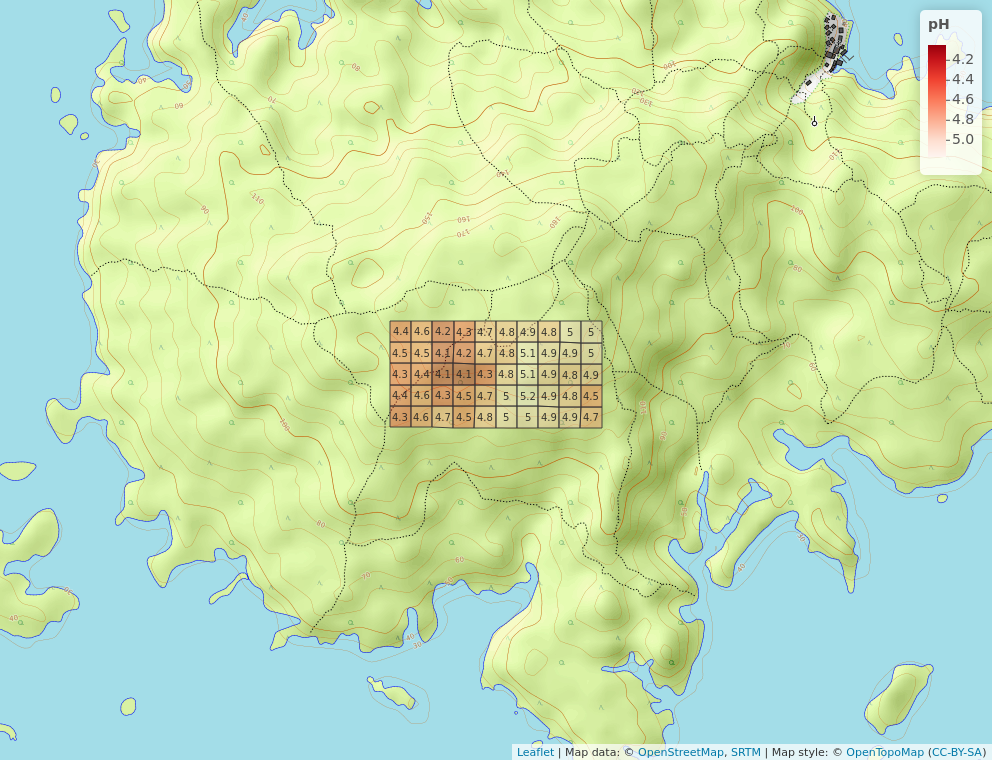
\includegraphics[width=1.00000\textwidth]{mapa_cuadros_ph.png}
\caption{mapa de la Isla Barro Colorado cuadros ph\label{fig:bci_map}}
\end{figure}

Como se puede ver, el PH es eminentemente ácido, en una pacerla de 50
Ha, la familia de plantas que nos interesa sobreabunda en estas
condiciones. Muy probablemente las familias de moraceae presentes en
otros lugares prosperen bajo condiciones muy diferentes, de como se
muestra en este mapa. Sin embargo los lugares a una misma latitud en el
planeta, se caracterizan por operar sobre los indiviuos bajo las mismas
condiciones, por ende las condiciones de PH en otras regiones tal vez no
se alejen tanto de las que por el momento se citan en el mapa. El PH es
un factor que en lo adelante incidirá en la utilidad de la planta,
especialmete a nivel comercial, la presencia de uno o varios elementos,
o la ausencia de estos determinará el valor utilitario de estas. La
quimiotaxonomía o qimiosistemática evalúa la presencia de elementos
químicos en especies vegetales, el aspecto químico de la clasificación
de las plantas, se basa en sus constituyentes es decir en sus
características moleculares. estas al igual que las características
geomorfológicas son controladas químicamente. Dentro los factores físico
químicos las medidas de PH no suelen presetar cambios significativos, en
las inmediaciones de las aguas del Canal de Panamá, pese a que se
presentan ligeras fluctuaciones en las medidas de este indicador, que en
esencia muestran la sensibilidad de las aguas circundantes, este por lo
general es regular (Simmonds, Gómez, \& Villalaz, 2002,). Esto sugiere
un grado de apatabilidad bastante desarrollado por las especies de la
familia en cuestión, no solo al medio de la isla, sino tambien de las
áreas circundantes. La fenología reprodctiva de la Isla de Barro
Colorado ha sido descrita extensamente por algunos autores. Los árboles
más grandes presentan un pico de floración entre febrero y junio, y
alcanzan un máximo en marzo y abril, justamente al final de la estación
seca (Williams-Linera \& Meave, 2002,). Tal vez este régimen de
floración y de adaptación permitan a las Moraceae mantener una fenología
por encima de los patrones físico químicos, en este caso especialmente
el PH.

En el mapa de abundacia global se advierten valores no lejanos de lo
ideal cuando se emplean parámetros de la muestra comprendidos entre 3600
y 5000, que en este caso sería una escala, en una parcela de 50 Ha. El
Valor promedio que representaría cada Ha en una media hipotética sería
de aproximadamente casi 4000 individuos de esta familia, sin embargo
tiende a cambiar cuando hablamos de riqueza. Si bien existen dentro de
esta familia, especies representativas de casi todas las formas de vida
leñosas, las formas más comunes entre las especies de bibosi, son por un
lado plantas hemiepífitas estranguladoras o matapalos y por otro,
plantas no epífitas con sistema propio de sustento o higuerones
(Fredericksen et al., n.d.,).

\begin{figure}
\centering
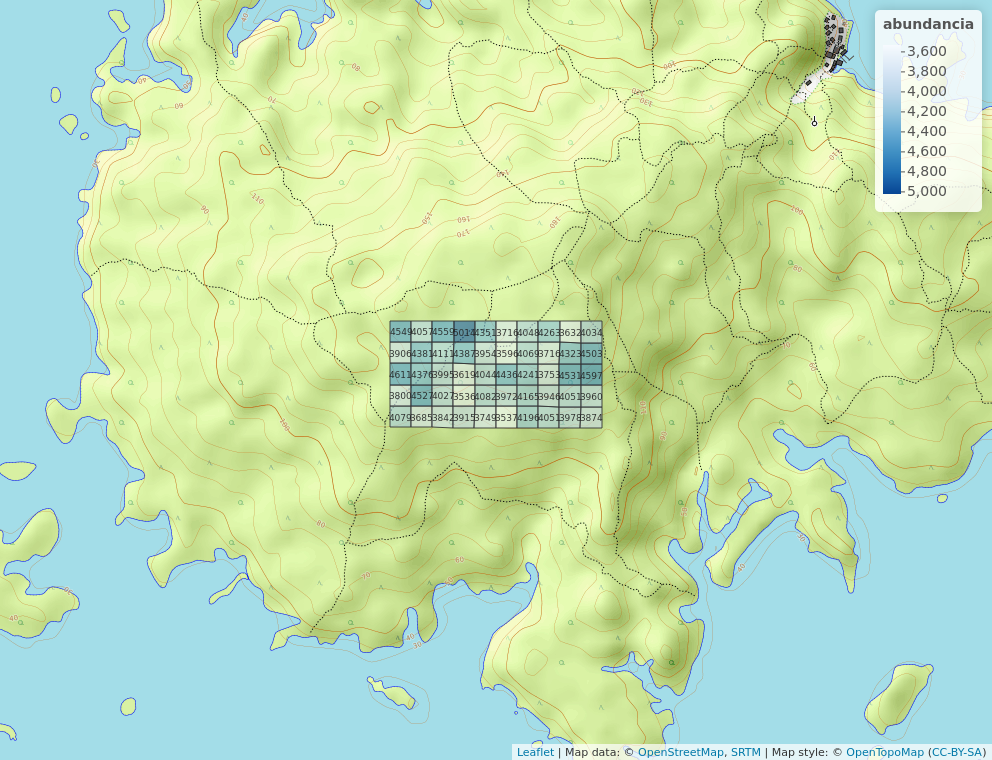
\includegraphics[width=1.00000\textwidth]{mapa_cuadros_abun_global.png}
\caption{mapa de la Isla Barro Colorado abundancia global
\label{fig:bci_map}}
\end{figure}

En el mapa de abundancia de mi familia no se presenta tampoco que la
muestra por hectárea se aleja de forma marcada del parámetro empleado
para la parcela de 50 Ha, en este caso en un parámetro de entre 200 y
700 individuos, podría verificarse una especie de relación directa entre
el primer y segundo mapa. En ambos casos cada Ha, adquiere valores
próximos a la dimensión numérica de individuos presentes en la parcela:

\begin{figure}
\centering
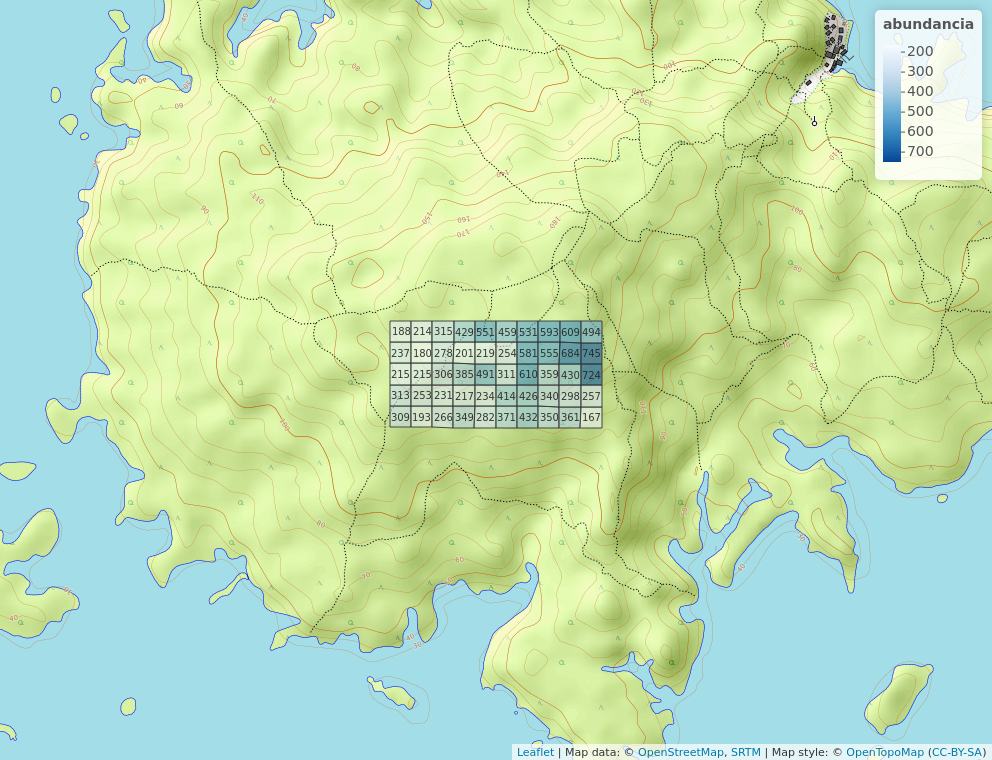
\includegraphics[width=1.00000\textwidth]{mapa_cuadros_abun_mi_familia.png}
\caption{mapa de la Isla Barro Colorado abundancia de mi familia
\label{fig:bci_map}}
\end{figure}

Como puede corroborarse existen muchos individuos, en este caso citando
la abundancia, de una determinada especie de la familia de Moraceae en
una Ha de la Isla Barro Colorado lo que muestra una amplia densidad para
una parcela de 50 Ha. Siendo estas plantas muchas veces ejemplares de
gran dimensión en muchos de los casos, se infiere que estas forman un
dosel impenetrable, típico de muchos bosques de la selva tropicla
centroamericana, en donde BCI no es la excepción. No solo estaríamos
hablando de Moraceae, sino de otras especies que forman la cubierta de
esta región intertropical.

Panamá es uno de los paises más diversos, ya que tiene el 10\% de la
fauna y flora global. México tiene el 11\%, pero Panamá cabe en México
unas 26 veces. Panamá tiene 1010 especies registradas, de esa cantidad
un tercio le corresponde a Barro Colorado. El bosque de Barro Colorado
se cierra muy abajo y es difícil ver algunas especies de aves, solo se
pueden escuchar. Las especies de Moraceae por lo general corresponden a
árboles de hojas anchas (latifoliados), lo que hace de los suelos de
estas especies, lugares prácticamente impenetrables por la radiación
solar, algo típico de la selva en cualquiera de sus denominaciones. En
el bosque la temperatura promedio es de 27 grados centígrados
(80\(^\circ\) fahrenheit), y la humedad es bastante alta. Otro factor
que incidirá sobre este tipo de angiospermas, es el de la pendiente del
terreno. La isla de Barro Colorado constituye uno de los ecosistemas más
grandes del mundo, lo que deja al descubierto la gran adaptabilidad que
presentan algunas plantas a este medio. Por tratarse de un lugar
sumamente pequeño, los rasgos orográficos han de ser casi
imperceptibles, pero sobre todo la edad de la isla no la hace poseedora
de formas del relieve que estén consolidadas dentro de lo ques es la
periodización geológica. Pues la isla se formó hace algo más de un
siglo, tiempo en el qe no caben eventos geológicos trascendentales. En
el mapa de pendientes citado anteriormente se pueden visualizar estos
menudos contrastes.En las curvas de nivel se pueden apreciar los valores
pequeños de altitud, lo que de un modo u otro favorece a estas familas.
La isla de Barro Colorado es realmente joven dentro de lo que es la
escala de tiempo geológica, solo tiene algo más de 100 años de
existencia lo que nos advierte de un relieve poco accidentado, debido en
gran parte a su tamaño, pero sobre todo a su edad. En este sentido sería
bueno apreciar las pendientes, y ver el valor de la altitud en esta
especie de enclave marítimo, lo que también favorece la existencia
abundante de ejemplares de Moraceae.

Ver mapa de pendiente\ref{fig:pendiente BCI}

\begin{figure}
\centering
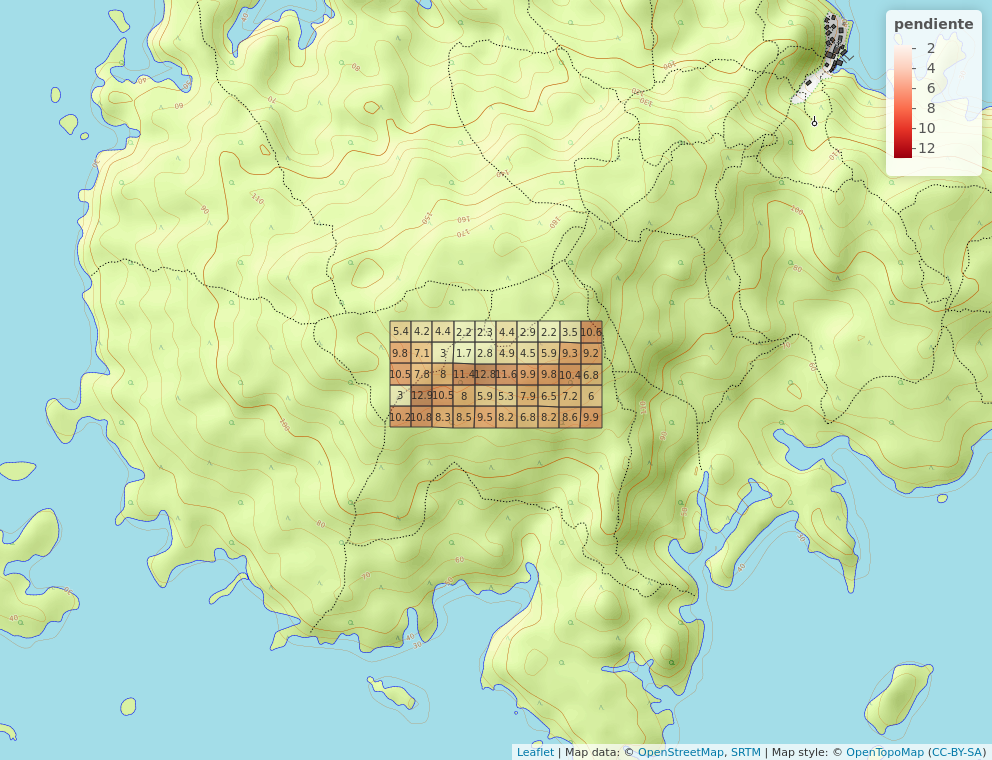
\includegraphics[width=1.00000\textwidth]{mapa_cuadros_pendiente.png}
\caption{mapa de la Isla Barro Colorado cuadros y pendientes
\label{fig:bci_map}}
\end{figure}

Para una consideración genral de la parcela de 50 Ha se destaca gran
pendiente, lo que es favorable para formaciones boscosas como la que nos
compete, aunque inservibles para la agricultura bajo cualquier
consideración que se haga a favor de la vegetación que no sea referente
a la anteriormente citada. Sin embargo la altitud guarda una relación
acorde con las dimensiones de la isla. Las plantas como las Moraceae
mantienen una relación favorble con estos grados de inclinación del
terreno. Ya en espacios controlados y con plantaciones con las qe se
persigue un determinado propósito se tiene un conocimiento sobre el
manejo de la pendiente, a sabiendas de que en este escenario han crecido
de forma silvestre sin intervención alguna de la mano del hombre. BCI
constituye como una especie de interrupción del sistema orgráfico de
zona istmica panameña y centroamericana, pues la espina dorsal de toda
la costa del Pacífico, aunque no se eleva de forma tan imponente como en
los Andes o en las Montañas Rocosas, en Centro America poseen
continuidad, aunque con una escasa altiud. Es como si se tratara de un
lugar construido para la investigación, en medio de sistemas tan
extremos, es decir franja estrecha de tierra y masas imensas de agua que
aguardan a ambos lados del Canal de Panmá (situación ístmica). En la
Isla de Barro Colorado la altura sobre el nivel del mar es pequeña, eso
reflejan las curvas de nivel presentes en los mapas anteriores.

En el caso de las variables ambientales numéricas se obtiene los
siguientes valores:

\begin{figure}
\centering
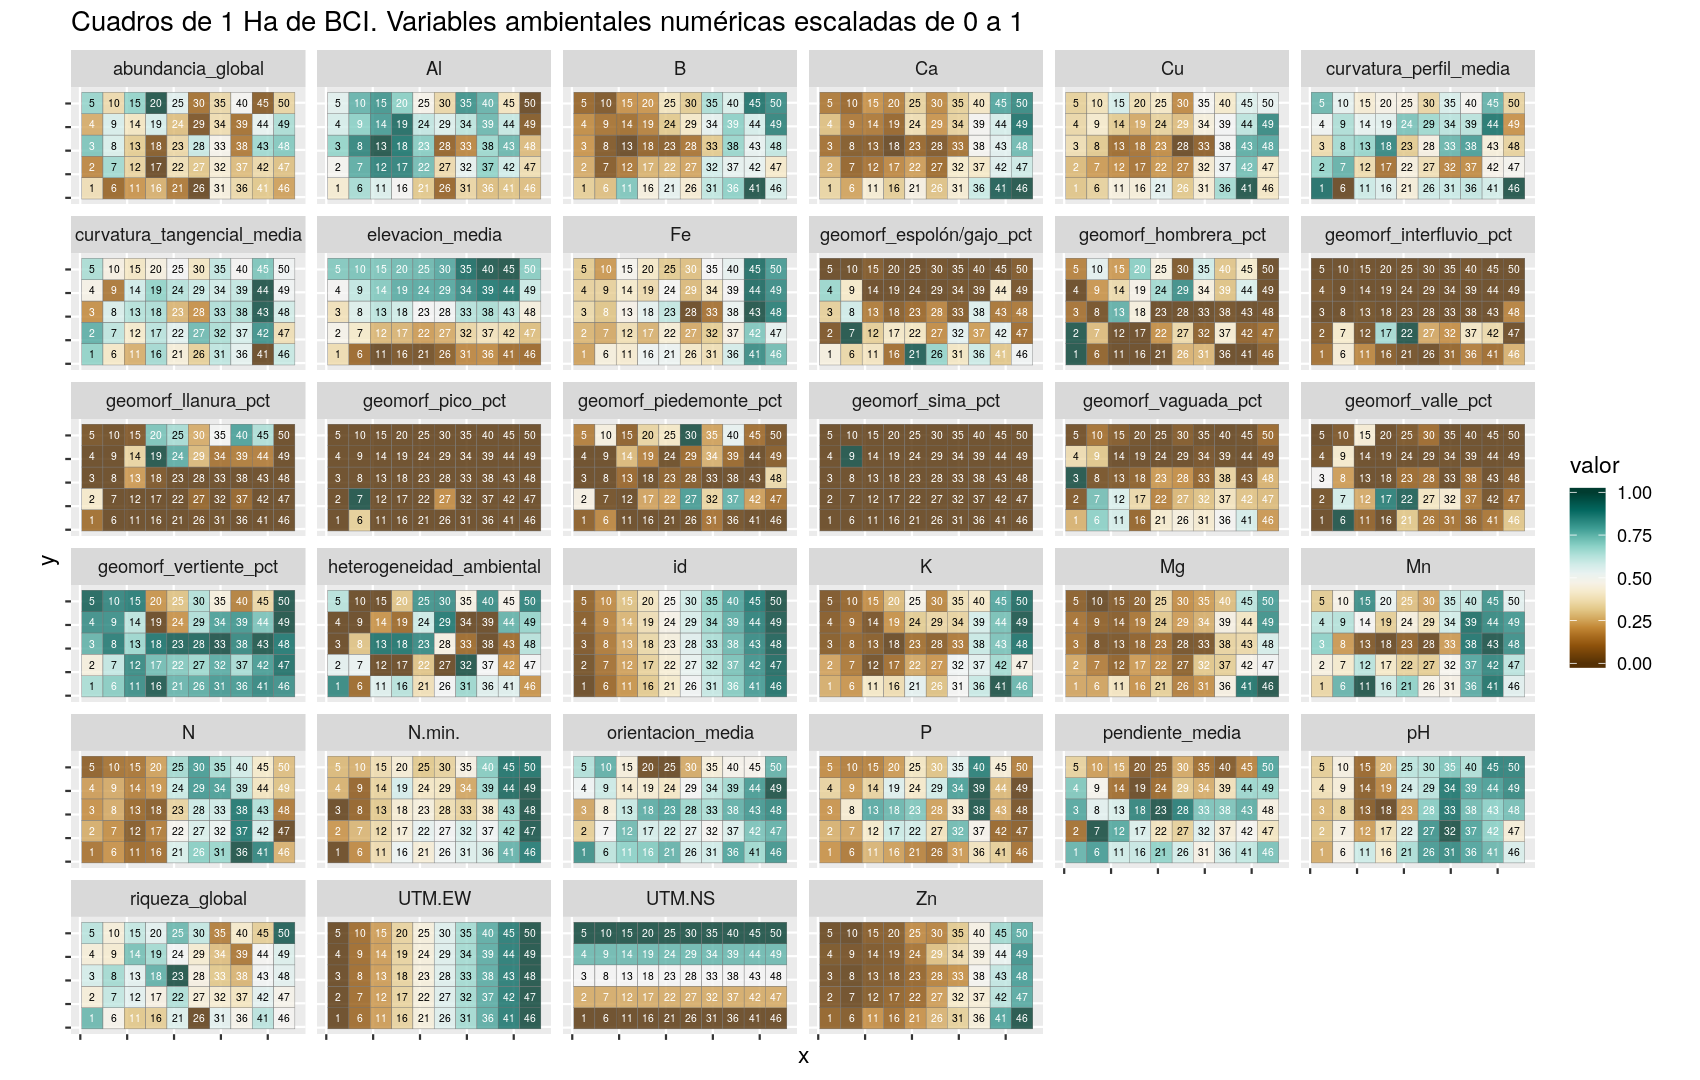
\includegraphics[width=1.00000\textwidth]{mapas_variables_ambientales_numericas.png}
\caption{mapa de la Isla Barro Colorado variables ambientales numéricas
\label{fig:bci_map}}
\end{figure}

Aquí podemos ver una especie de síntesis de las informaciones que
ofrecen las variables ambientales de una Ha, escaladas de 0 a 1. En el
caso de las geoformas, correspondientes a llanuras, se obtienen valores
grandes en un segmento de la escala que va de 0.00 a 0.25, lo que
refleja un terreno eminentemente llano.

Con relación a las vrtientes ocurre todo lo contrario, se obtienen
valores grandes, en el segmento de la escala que va de 0.75 a 1.00, lo
que se refiere a mayor inclinación en contraste con las tierras llanas.

Otra geoforma como es el caso de los valles, presenta valores muy
pronunciados en los segmentos bajos de la escala citada, por ende se
puede inferir que las tierras bajas son predominantes por encima de las
tierras altas. Los valores de la escala muestran amplias diferencias
entre unas variables y otras, pero dentro de la misma escala, suele
verse la superioridad de una sobre otra.

Al estar dispuestas en el primer cuadrante de un plano bidimensional,
algunas variables por Ha, presentan mayores valores en X que en Y, y
viceversa. Sería esa una forma inteligente de ver el comportamiento de
las variables con realación a los ejes X e Y. Lo mismo que en los mapas
de riqueza, tanto de la familia como global, puede verse la
superioridad, de un bosque que corresponde a la formación vegetal tipo
selva, propio de regiones tropicales, intertropiclaes, y ecuatoriales,
desde luego con algunas variaciones por cuestiones de latitud.

A continuación el mapa de variables ambientales nominales

\begin{figure}
\centering
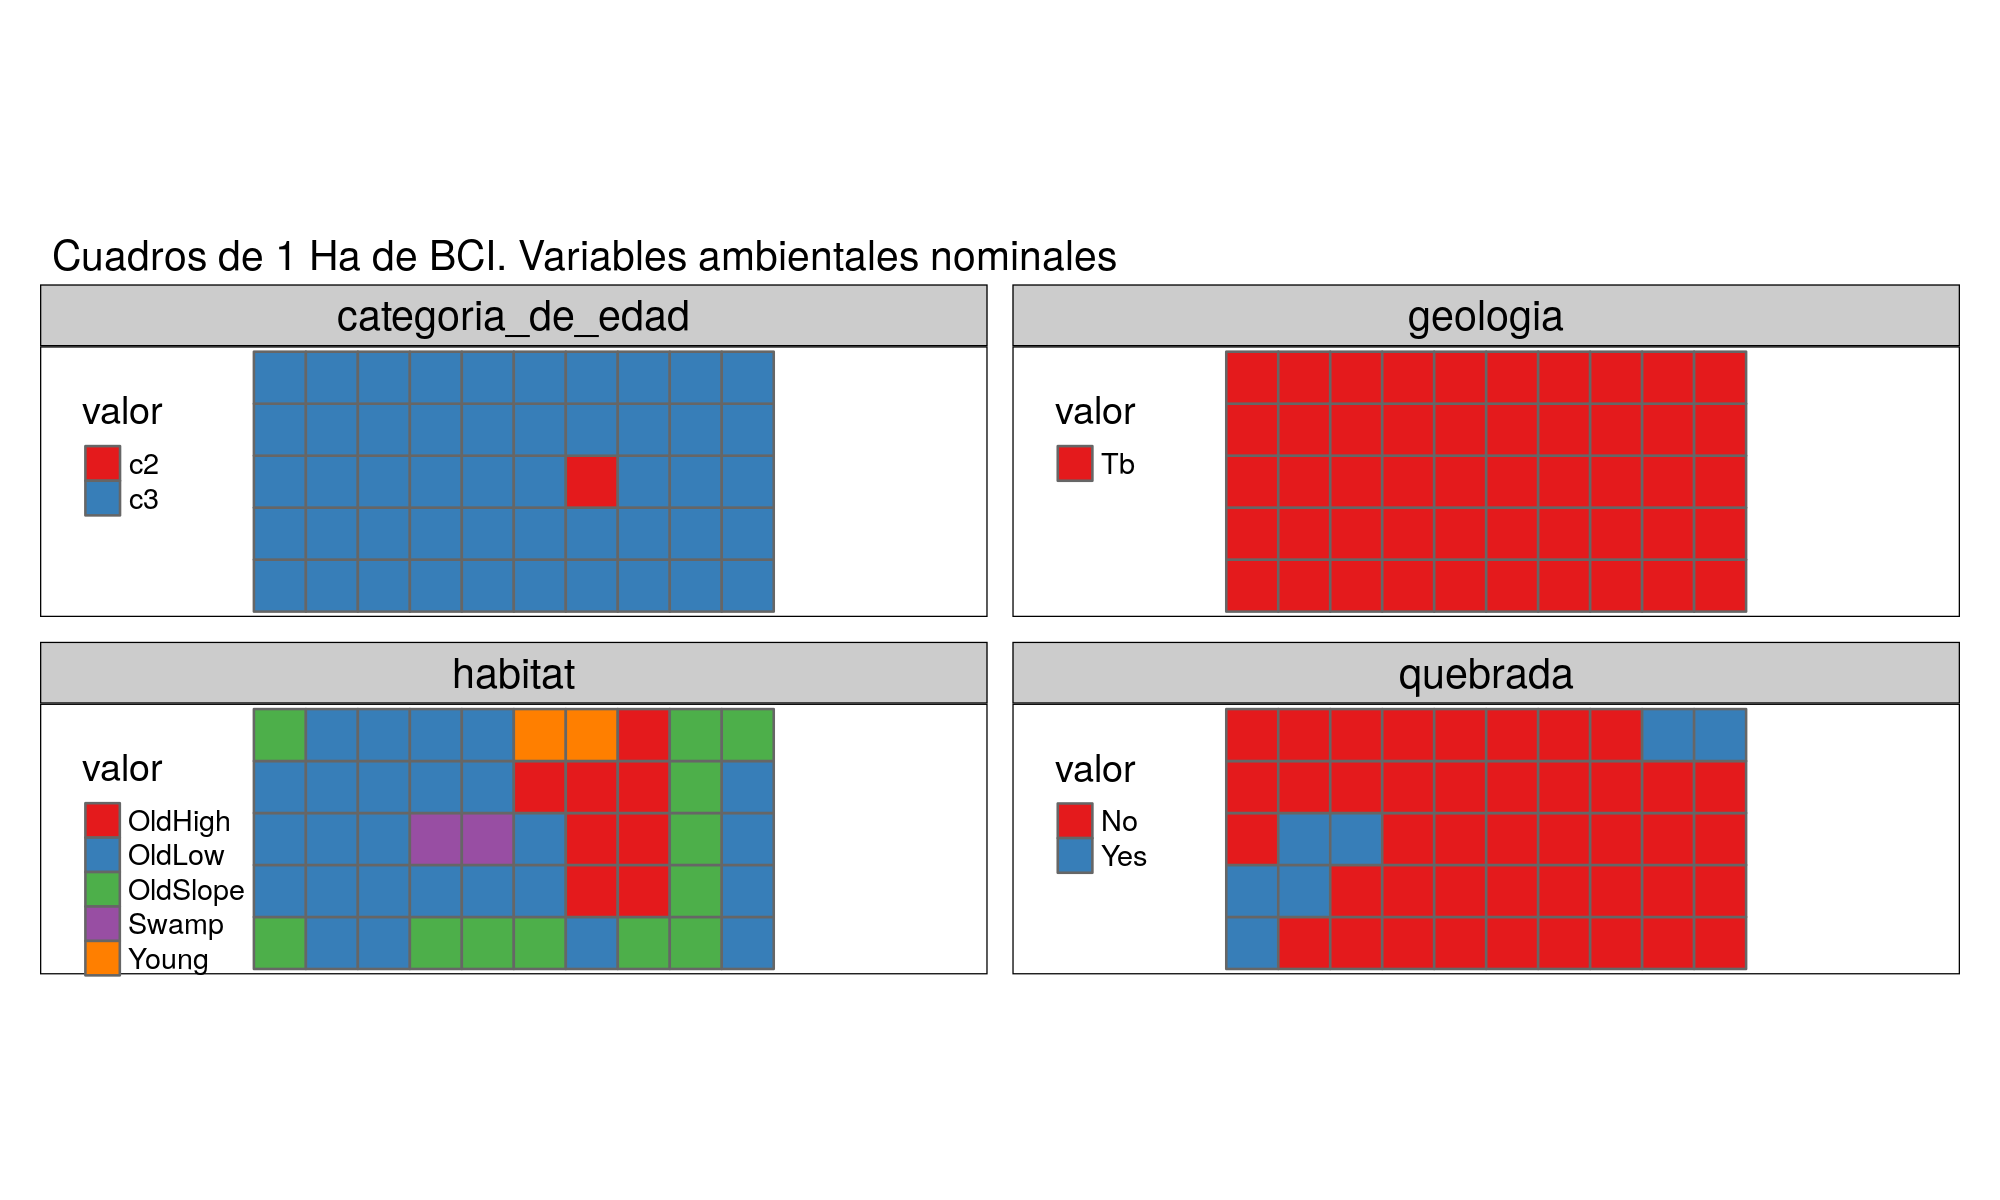
\includegraphics[width=1.00000\textwidth]{mapas_variables_ambientales_nominales_tmap.png}
\caption{mapa de la Isla Barro Colorado variables ambientales nominales
\label{fig:bci_map}}
\end{figure}

Aquí se distingue variables como la categoría de edad, geología de la
zona, hábitat, y la quebrada. El hábitat de bosque viejo en terreno alto
(OldHigh), se destaca por su relativa minoría. En tanto que el bosque
viejo en relieve bajo (OldLow) es el más abundante. El bosque viejo con
pendiente (OldSlope), es relativamente abundante. El pantano es escaso
(Swamp), así también el bosque joven (Young). En cuanto a la geología
tenemos que el tipo de roca predominante es de tipo intrusivo o
plutónica. Las quebradas o barrancos son estrechos. Existen dos grandes
categorías dentro de la variable de edad, el bosque viejo en terreno
bajo, y el bosque viejo en terreno alto. De lo anterior se infiere que
existe más terreno bajo con bosque viejo en BCI en una base gelógica
joven, que con las demás variables. El mapa de riqueza presenta un
formato similar a los de abundancia, con comportamientos diferenciados
por Ha, comparados con la parcela de 50 Ha. En el siguiente mapa puede
apreciarse la riqueza de la famiia botánica bajo estudio (Moraceae) por
Ha:

\begin{figure}
\centering
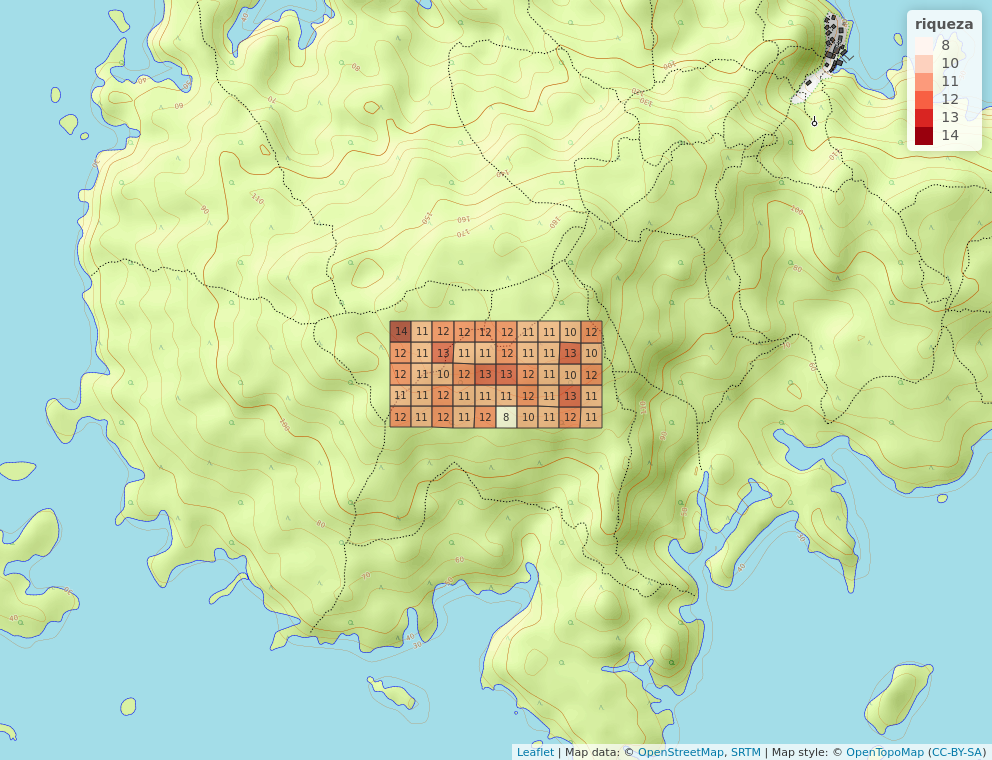
\includegraphics[width=1.00000\textwidth]{mapa_cuadros_riq_mi_familia.png}
\caption{mapa de la Isla Barro Colorado cuadro de riqueza mi familia
\label{fig:bci_map}}
\end{figure}

En esta parte puede apreciarse que la riqueza es casi la misma por Ha,
acercándose al nivel superior de la escala, así se puede asumir que el
grado de dispersión de algunos individuos de la familia Moraceae es casi
nulo. Existe una gran riqueza de estas plantas que ayudan en gran parte
a mantener este gran ecosistema. Sin lugar a dudas puede apreciarse la
inmensa riqueza que hay en BCI por hectárea, solo concerniente a
Moraceae, formando un tapiz casi perfecto, de individuos distintos de
una misma familia. Ya para el mapa de riqueza global se advierten
mayores contrastes por hectárea, pero igual se impone la diversidad, la
multiplicidad de individuos es asombrosa.

\begin{figure}
\centering
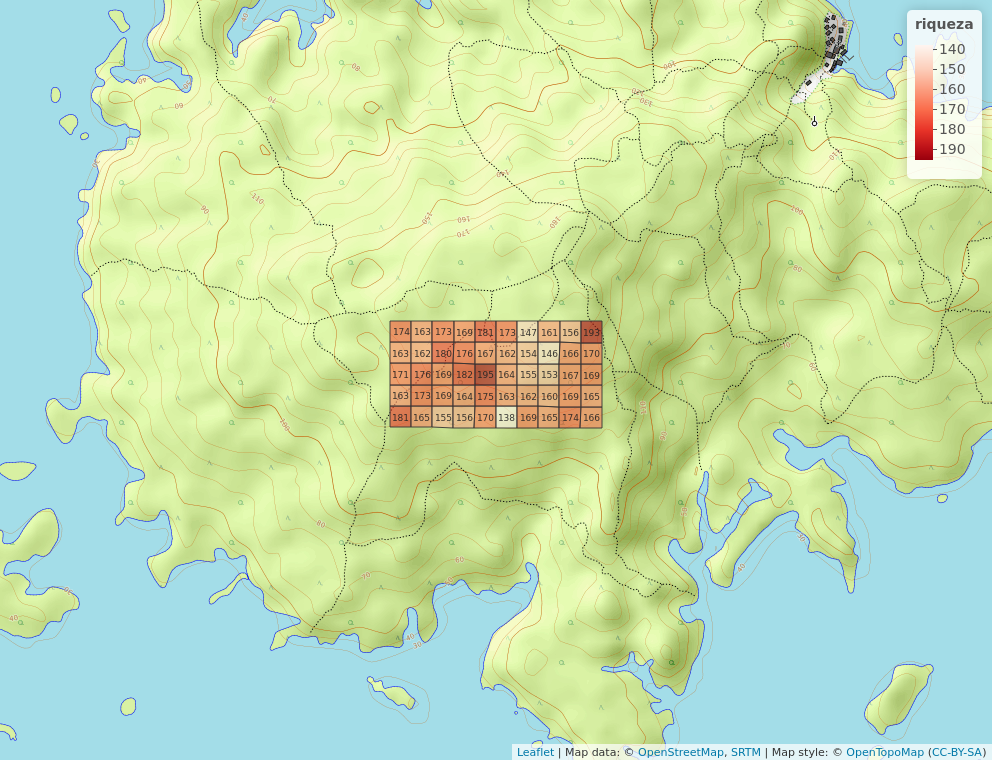
\includegraphics[width=1.00000\textwidth]{mapa_cuadros_riq_global.png}
\caption{mapa de la Isla Barro Colorado riqueza global
\label{fig:bci_map}}
\end{figure}

Como se pudo ver en los mapas, y los cuadros de variables, la Isla de
Barro Colorado presenta gran riqueza y abundancia en espacios muy
reducidos, especialmente de la familia de las Moraceae. Todo esto nos
hace pensar que se trata un gran bioma en miniatura en el que se reducen
las distancias, y se incrementan los ejemplares que hacen confluir la
biología y la geografía. Tal vez en el aspecto geomorfológico no se
puedan hacer conjeturas similares. Pero desde la biogeografía, el
sendero es complejo. El hecho de que exista este conglomerado de
especies de plantas y animales, requiere de unas condiciones óptimas
para hacer posible la vida de este gigantesco ecosistema. En los mapas
de abundacia, tanto global como de la familia se advierte un crecimiento
casi perfecto, bajo condiciones físicas y químicas que le son favorables
a la vida en esta parte del mundo.

No se ignora que a la misma latiud se encuetren condiciones similares en
otros rincones de la tierra, de hecho las zonas intertropicales, las
tropicales y las ecuatoriales se caracterizan más por la riqueza que por
la abundancia. Pero en ese sentido tenemos millones de kilómetros bajo
estudio si nos adentraramos en las grandes selvas que se conocen de
antiguo, y tal vez nos toparíamos más con abundancia que con riqueza.
Las grandes expediciones de la historia se han distinguido siempre por
cubrir amplios itinerarios, que a su vez implican grandes distancias. En
ese sentido nunca dejaríamos de mencionar a Darwuin, Humboldt, y otros
investigadores que no fueron merecedores de las ventajas de esta aldea
global que ha venido a simplificarlo todo, aunque no todos estamos
inmersos en ese pequeño nicho cibernético. En los cuadros de variables
ambientales, se corroboran las diferencias entre unas y otras, se
distinguen tierras bajas de otras no muy altas. Pero no solo se analizan
los rasgos geomorfológicos, otras variables ofrecen tambien allí su
concurso. Aprecen valores de PH, riqueza global por igual, abundancia
global, entre otras variables.

En esta parte se aborda lo que es la medición de asociación, tomando en
cuenta lo que son los valores de disimilaridad o distancia, así como las
matríces de correlación. Dentro de los modelos de medición de asociación
existen los modos Q y R, en este caso de la distancia o disimilaridad,
tenemos el modo Q que describe la distancia entre objetos cuantitativos.
La paradoja de Orlóci plantea que la distancia euclidea es más pequeña
entre sitios que no comparten especies que entre sitios que sí las
comparten. A continuación se presenta una matríz de disimilaridad.

\begin{figure}
\centering
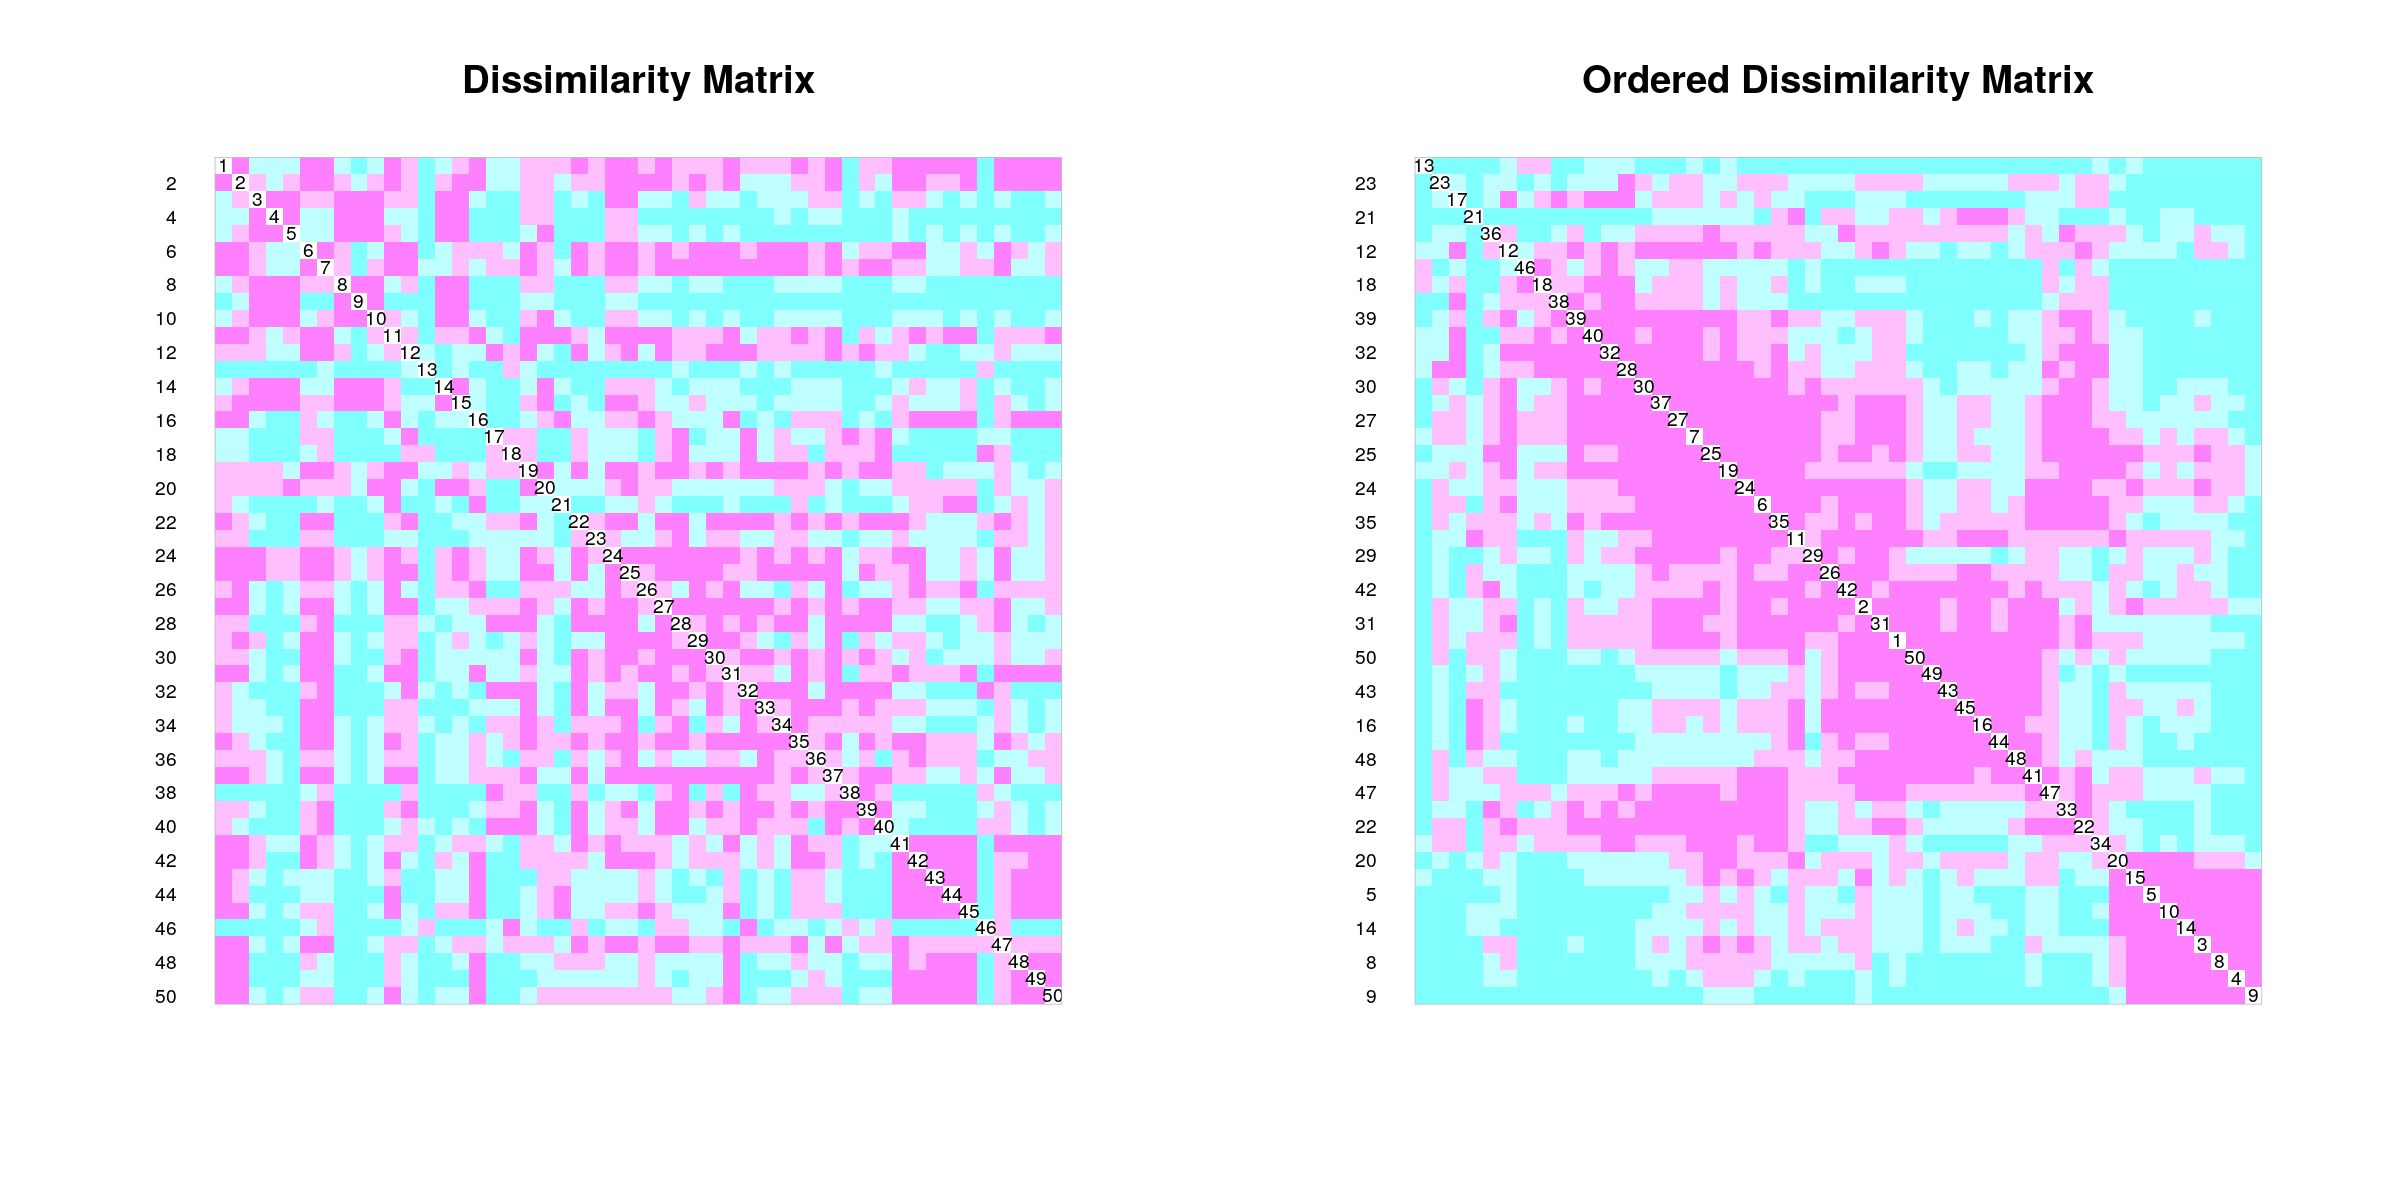
\includegraphics[width=1.00000\textwidth]{matriz_disimilaridad_hellinger.png}
\caption{mapa de la Isla Barro Colorado matriz disimilaridad hellinger
\label{fig:bci_map}}
\end{figure}

La matrz de disimilaridad es es una representación de la medición de
asociación entre objetos en el modo Q, como serían los sitios de
muestreo. En esta matriz se puede apreciar una fuerte asociación entre
objetos y esto lo indica la continuidad del color rosado (cuadro de la
derecha). En este caso nos referimos a la matriz de la derecha, que es
la matriz ordenada, a partir de la primera. Por ejemplo entre los sitios
40 y 35 existe una distancia muy pequeña entre sitios parecidos para la
matriz ordenada. La transformación Hellinger permite hacer la
interpretación en base a dos colores representativos: Color fucsia
(magneta, rosa) que equivale a corta distancia, muy similar, y el cian o
celeste que significa gran distancia o poco similar, todo esto con
relación a los elementos de la familia de las moraceae. Algunos de los
valores de disimilaridad o de distancia entre objetos que podemos
apreciar dentro de la transformación Hellinger son los siguientes: Entre
los sitios 2 y 1, tenemos que la distancia (dbl) es de 0.187, entre 3 y
1 es de 0.439, entre 4 y 1 es de 0.499, entre 5 y 1 es de 0.430, entre 6
y 1 de 0.297, entre 7 y 1 es de 0.280, entre 8 y 1 es de 0.492, entre 9
y 1 es de 0.584, entre 10 y 1 es de 0.425, y entre 11 y 1 es de 0.269 lo
que revela una escasa distancia o disimilaridad entre los objetos.

A continuación presento una versión mejorada de la matríz ordenada de
datos cuantitativos de especies (abundancia) con fuerte asociación en la
diagonal.

\begin{figure}
\centering
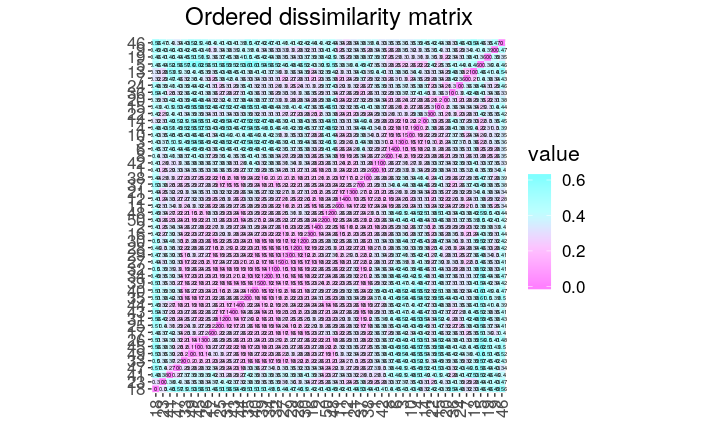
\includegraphics[width=1.00000\textwidth]{matrizdedisimilaridad.png}
\caption{mapa de la Isla Barro Colorado matriz disimilaridad
\label{fig:bci_map}}
\end{figure}

En esta matriz de disimilaridad o de distancia vienen a recrearse los
anteriores casos de abundancia de los mapas de la Isla de Barro
Colorado. En la diagonal se pueden apreciar los sitios que poseen
características similares con la menor distancia(color rosado), mientras
que en los demás lugares se aprecian lugares con características
similares a mayor distancia y con una menor asociación (color cian o
celeste). Hasta el momento me he centrado en el modo Q que mide el nivel
de asociación por medio de la disimilaridad o similiridad. Algo
sumamente importante dentro del modo Q, en este caso basándome en datos
binarios (presencia/ausencia) es la famosa distancia de Jaccard, la
misma se puede expresar como la proporción de especies no compartidas.
Para el caso correspondinte de los datos de moraceae, la distancia (dbl)
muestra los siguientes resultados para algunos sitios: Entre 2 y 1, la
distancia es de 0.22, para 3 y 1 es de 0.33, entre 4 y 1 es de 0.222,
para 5 y 1 es de 0.3, para 6 y 1 es de 0.333, para 7 y 1 es de 0.222,
para 8 y 1 es de 0.333, para 9 y 1 es de 0.333, para 10 y 1 es de 0.4, y
para 11 y 1 es de 0.333, evidenciando en este caso una fuerte
asociación.

La similaridad es la proporción de datos compartiods entre sitios, en la
siguiente gráfica de la matriz pueden apreciarse las espcecies
compartidas entre sitios.

\begin{figure}
\centering
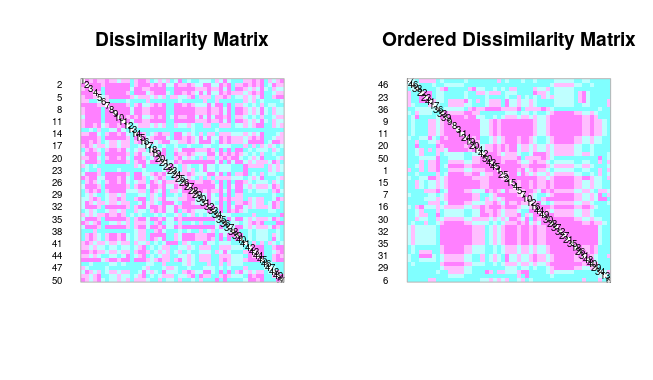
\includegraphics[width=1.00000\textwidth]{matriz_similaridad.png}
\caption{mapa de la Isla Barro Colorado matriz disimilaridad
\label{fig:bci_map}}
\end{figure}

Puede apreciarse en los bloques de colores las especies compartidas
entre sitios, y que son exclusivas de dichos sitios. Por ejemplo para
las variables a b y c, que se desprenden de la fómula de la similaridad,
donde a representa el número de especies compartidas, b es el número de
especies exclusivas del sitio 2 y c el numero de especies exclusivas del
sitio 1.

En el modo R se mide la asociación entre pares descriptores, es decir
variables o especies, mediante la covarianza y la correlación. Por
ejemplo para las variables a b y c, que se desprenden de la fómula de la
similaridad, donde a representa el número de especies compartidas, b es
el número de especies exclusivas del sitio 2 y c el numero de especies
exclusivas del sitio 1.

Un ejemplo ilustrativo sería el mapa de calor

\begin{figure}
\centering
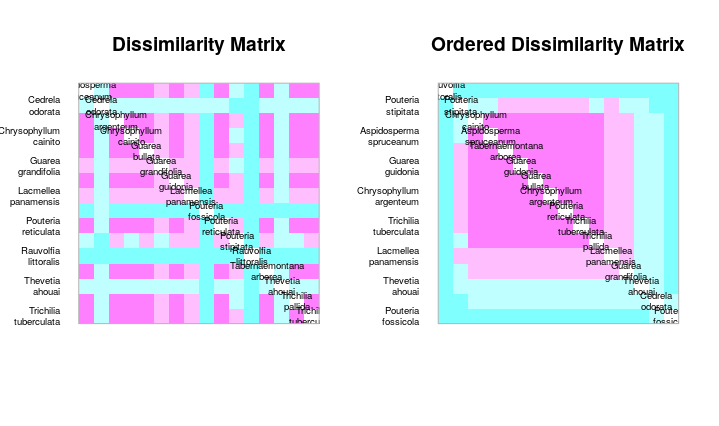
\includegraphics[width=1.00000\textwidth]{mapadecalor.png}
\caption{mapa de la Isla Barro Colorado mapa de calor
\label{fig:bci_map}}
\end{figure}

En el mapa de calor mostrado se muestra una relación de dependencia en
la diagonal de la derecha, esto es lo que se mide en el modo R, la
asociación entre elementos descriptores, en este caso la abundancia de
especies como variables. Entre la cainito aspidosperma y la trichinia
tuberculata se nota una fuerte dependencia, evidenciado por la
continuidad del color fucsia o rosa.

\section{Discusión}\label{discusiuxf3n}

La abundancia y riqueza de la familia Moraceae, dentro de la isla Barro
Colorado, es vieja y asentada en terreno bajo, en su generalidad, con
una adaptación bastante ajustada a las condiciones de los factores
físico químicos de dicha isla, por lo general son plantas perennes, de
gran porte que sirven de alimentación a los individuos frugívoros que
allí habitan, constituyendo con su dosel el típico paisaje de la selva
tropical crentroamericana.

Dentro de la selva del ístmo, BCI, es como un esctracto sintético
susceptible de múltiples investigaciones, por su amplia concentración de
flora y fauna. Si bien la Isla Barro Colorado es un enclave marítimo, y
de investigación científica, contando por ende con las riquezas antes
descritas, es motivo de cuestionamiento, el cómo un espacio, esta
pequeña isla, haya acumulado estas riquezas en tan poco tiempo, a
sabiendas de la zona geoastronómica en que se encuentra. Sería más
aceptable la abundancia.

Pero la construcción de riquezas ecológicas, ademas del emplazamiento
geográfico, requieren de eventos geológicos, geográficos y tal vez
antrópicos, en este caso tenemos el Canal de Panamá, el recuerdo mejor
conservado de la injerencia yanqui en el Caribe. Una isla que se formó
en algo más de un siglo, pues de la misma forma corre el riesgo de
desaparecer. Pero esto solo compete a un asunto geológico, que no
concierne a este trabajo, solo de manera parcial.

Nuestro interés se centra, en esta parte, en las condiciones que han
creado este espacio insular tan singular, en un tiempo tan breve, en el
istmo de Panamá. Si bien sabemos que América es la masa continental que
alcanza mayor extensión latitudinal, es probable que en todo el tiempo
precedente a la construcción del canal, se dieran las migraciones de
especies tanto del norte como del sur. Aunque, una vía interoceánica
artificial como lo es el Canal de panamá, probablemente no provocaría
cambios notables en el equilibrio biológico de las comunidades de
individuos que poblaban esta parte del continente.

La sostenibilidad de las especies de plantas y animales que allí existen
no se puede poner en duda, por las condiciones climáticas que en dicho
lugar se mantienen. Es como si tratara de un ambiente controlado y
planificado. De modo que las investigaciones siempre tienen una página
que arañar, dando motivos de colgarse una mochila y salir a hacer
trabajo de campo. Es muy probable que para muchos, BCI siga siendo el
secreto mejor guardado dentro de las zonas de investigación más
llamativas del mundo,lo cual resulta ser asombroso por el peso que posee
el istmo de de Panamá a escala comercial.

El presente artículo ha sido un intento por abordar la información
básica de la familia de las Moraceae, desde una perspectiva científica,
teniendo como escenario la Isla de Barro Colorado. En el desarrollo me
he volcado más en lo que es la distribución de individuos por ha, en una
parcela de 50 ha, tanto desde una perspectiva global, como específica,
en las condiciones del terreno, así como en la situación geográfica,
pretendiendo dar un enfoque lo más abarcador posible, siguiendo estas
variables, que han de ser de las más pertinentes para la consideración
de un trabajo de campo.

Sabemos que esta familia de angiospermas posee gran riqueza y abundancia
en esta parte del istmo, y que las condiciones típicas del suelo son
idóneas para su sostenimiento. En un principio mencioné el caso de
Mexico, por sus estadísticas en cuanto a predominio de plantas,
especialmete de la familia que estoy tratando, un basto territorio que
alberga todo lo que le permite su inmensa superficie. Sin embargo, BCI,
es otro Mexico tipo laboratoio destinado a la investigación.

Pero como dirían por ahí, la ciencia está en crisis y cada vez es más
pequño el número de hombres y mujeres que se interesan por escribir en
favor de la ciencia, de modo que para muchos estos lugares pasan
desapercibidos, y la existencia de plantas y animales como un trazo más
en un mural en el que no sale el sol, en el que no existe el dinamismo.
Pero no dejemos esto en manos de la pobalción, cedamos un poco a los
sistemas de gobierno que son los que generan los programas de educación,
y en ellos dejan cada vez menos espacio a la ciencia, una especie de
neocolonialismo.

Existen muchos lugares en el Mar Caribe que como BCI, pueden ser grandes
laboratorios, a partir de los cuales se pueda hacer ciencia, producir
material científico de utilidad, pero la dependencia es peor que el
analfabetismo. Por ello tal val tenemos una ciencia estacionaria,
incapáz de dar el santo de la libertad. En nuestro territorio, la
República Dominicana, han existido personajes que se han destacado en la
ciencia, pero siempre serán dominicnaos.

Y se espera que el caudal de inforamción que se generan en las
investigaciones alcance a estos lugares, porque la ciencia genera
identidad a los lugares y los hace crecer. BCI, tiene algo más de 100
años, pero Panamá como nación es más vieja, y no es mi incumbencia el
tema político, ni de este artículo. Pero hago la aclaración porque
entiendo que se puede crecer en la ciencia, siempre dejando claro que
cada pueblo tiene contextos distintos y que el error siempre será tratar
de copiar. Este ha sido un trabajo en virtud del interés biológico, y
geográfico. Esperando que sea del agrado de quienes puedan leerlo.

\section{Agradecimientos}\label{agradecimientos}

Quiero dedicar todo mi agradecimiento, primero a Dios porque es quien
hace posible todas las cosas, luego al maestro José Ramón Martínez
Batlle, maestro de la escuela de ciencias geográficas en la facultad
ciencias de la Universidad Autónoma de Santo Domingo, en las áreas de
biogeografía, geomorfología, y anteriormente de geología por enrutarnos
en este mar de investigación que siempre termina arrojando cosas nuevas.
Por último a mis compañeros de carrera, Carolain Pérez Ureña, Ana Hilda
Valera, Darihanna Linares y Wilson Robles Rosario, sin ellos esto no
habría sido posible, muchas gracias.

\section{Información de soporte}\label{informaciuxf3n-de-soporte}

\begin{figure}
\centering
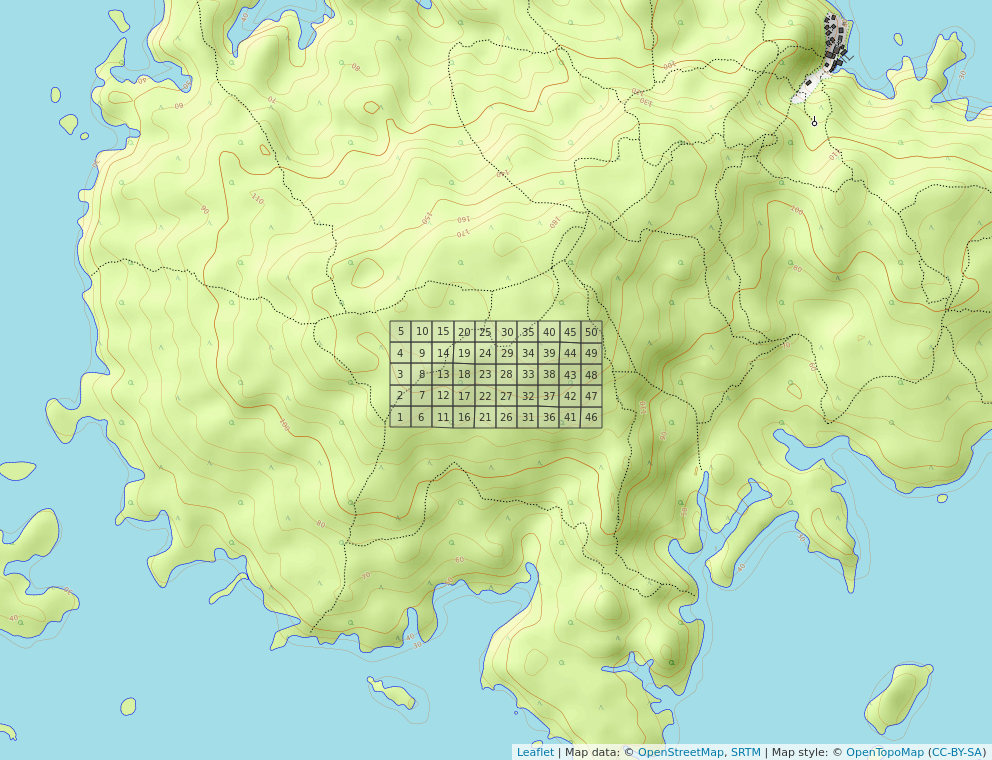
\includegraphics[width=1.00000\textwidth]{mapa_cuadros.png}
\caption{mapa de Isla Barro Colorado cuadros\label{fig:bci_map}}
\end{figure}

\begin{figure}
\centering
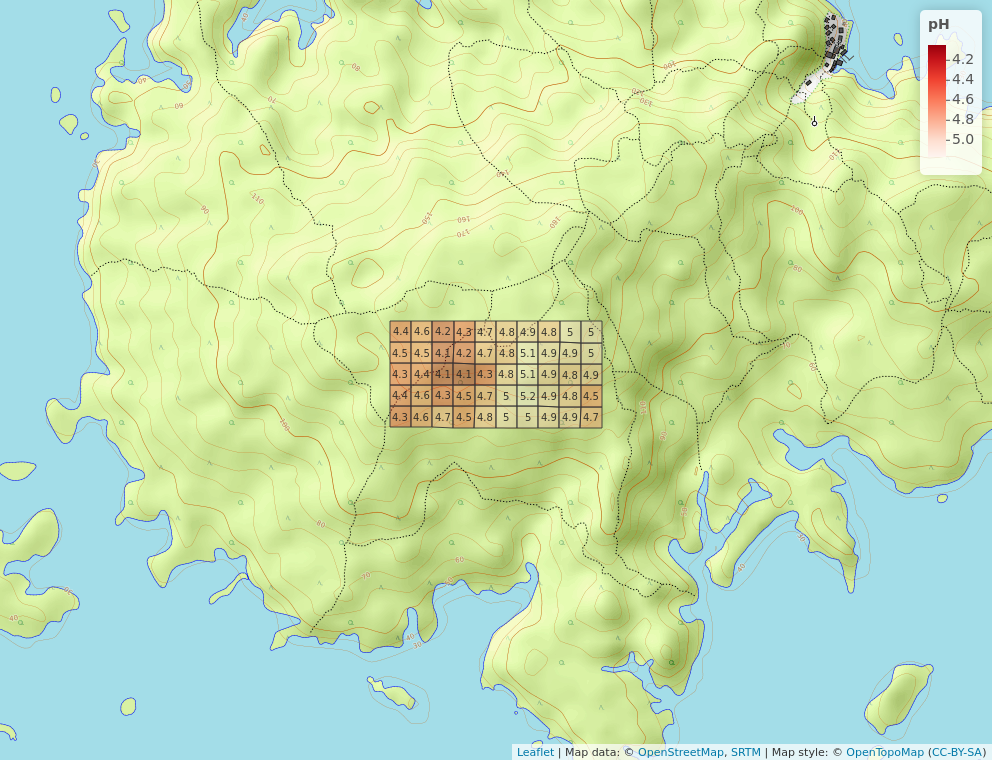
\includegraphics[width=1.00000\textwidth]{mapa_cuadros_ph.png}
\caption{mapa de la Isla Barro Colorado cuadros ph\label{fig:bci_map}}
\end{figure}

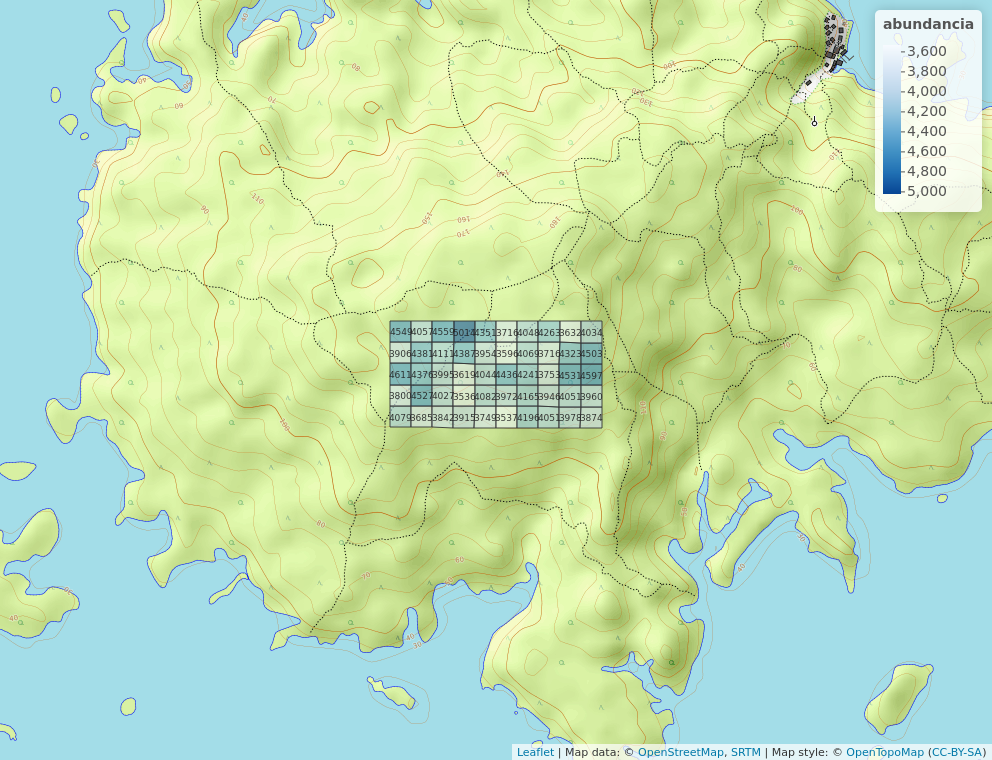
\includegraphics[width=1.00000\textwidth]{mapa_cuadros_abun_global.png}
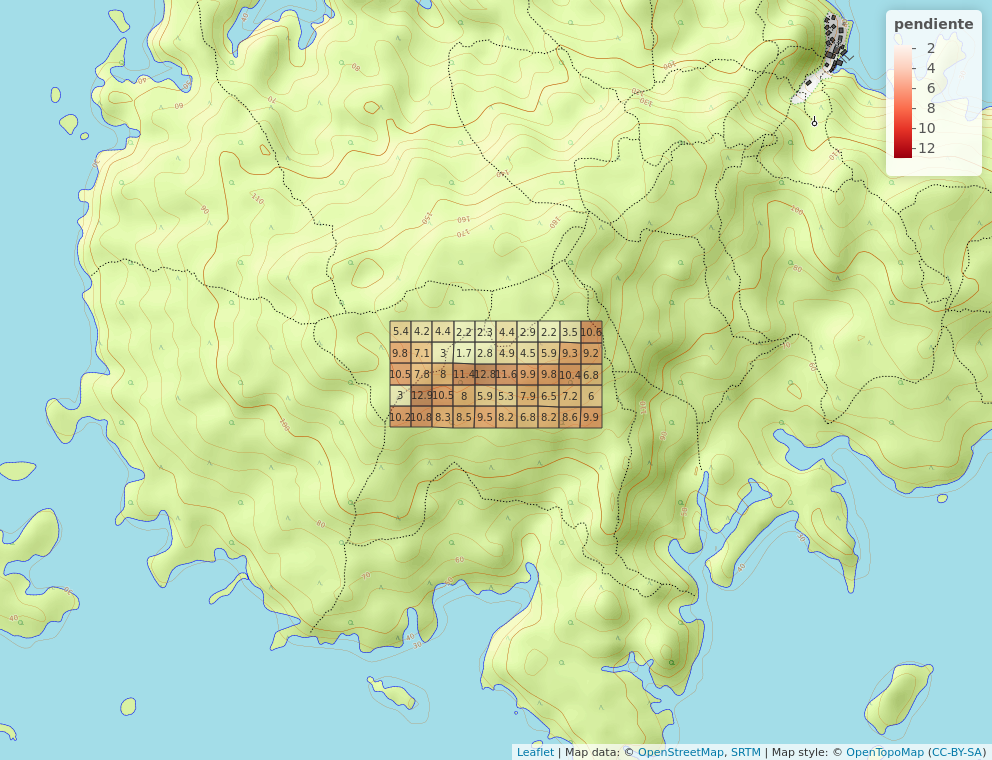
\includegraphics[width=1.00000\textwidth]{mapa_cuadros_pendiente.png}
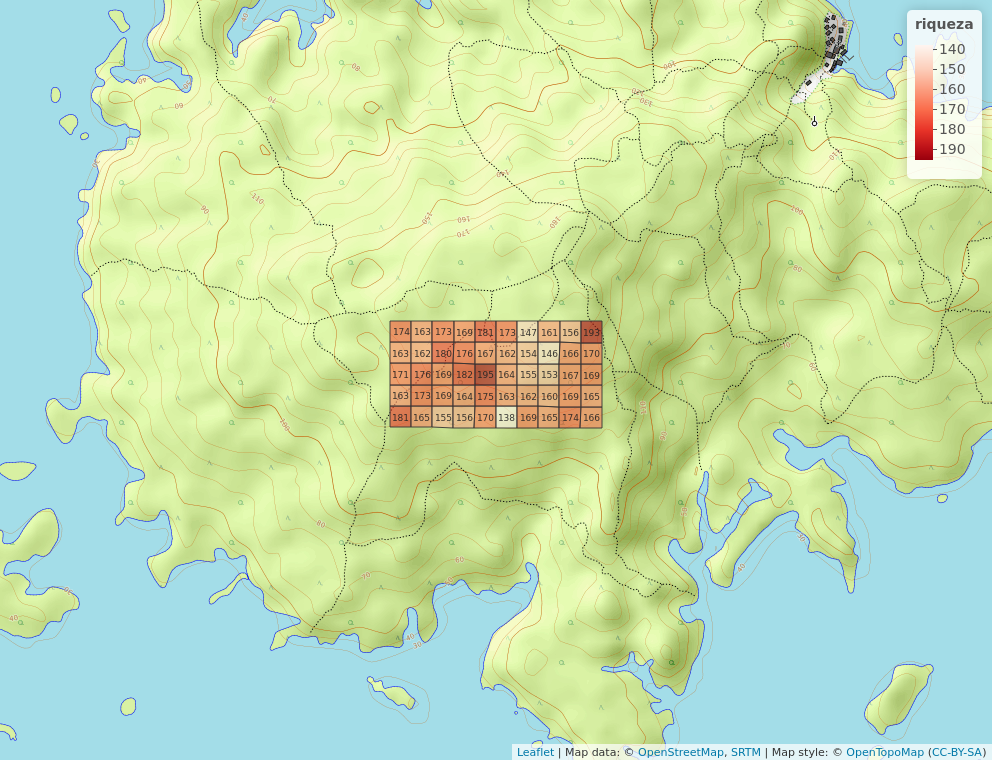
\includegraphics[width=1.00000\textwidth]{mapa_cuadros_riq_global.png}

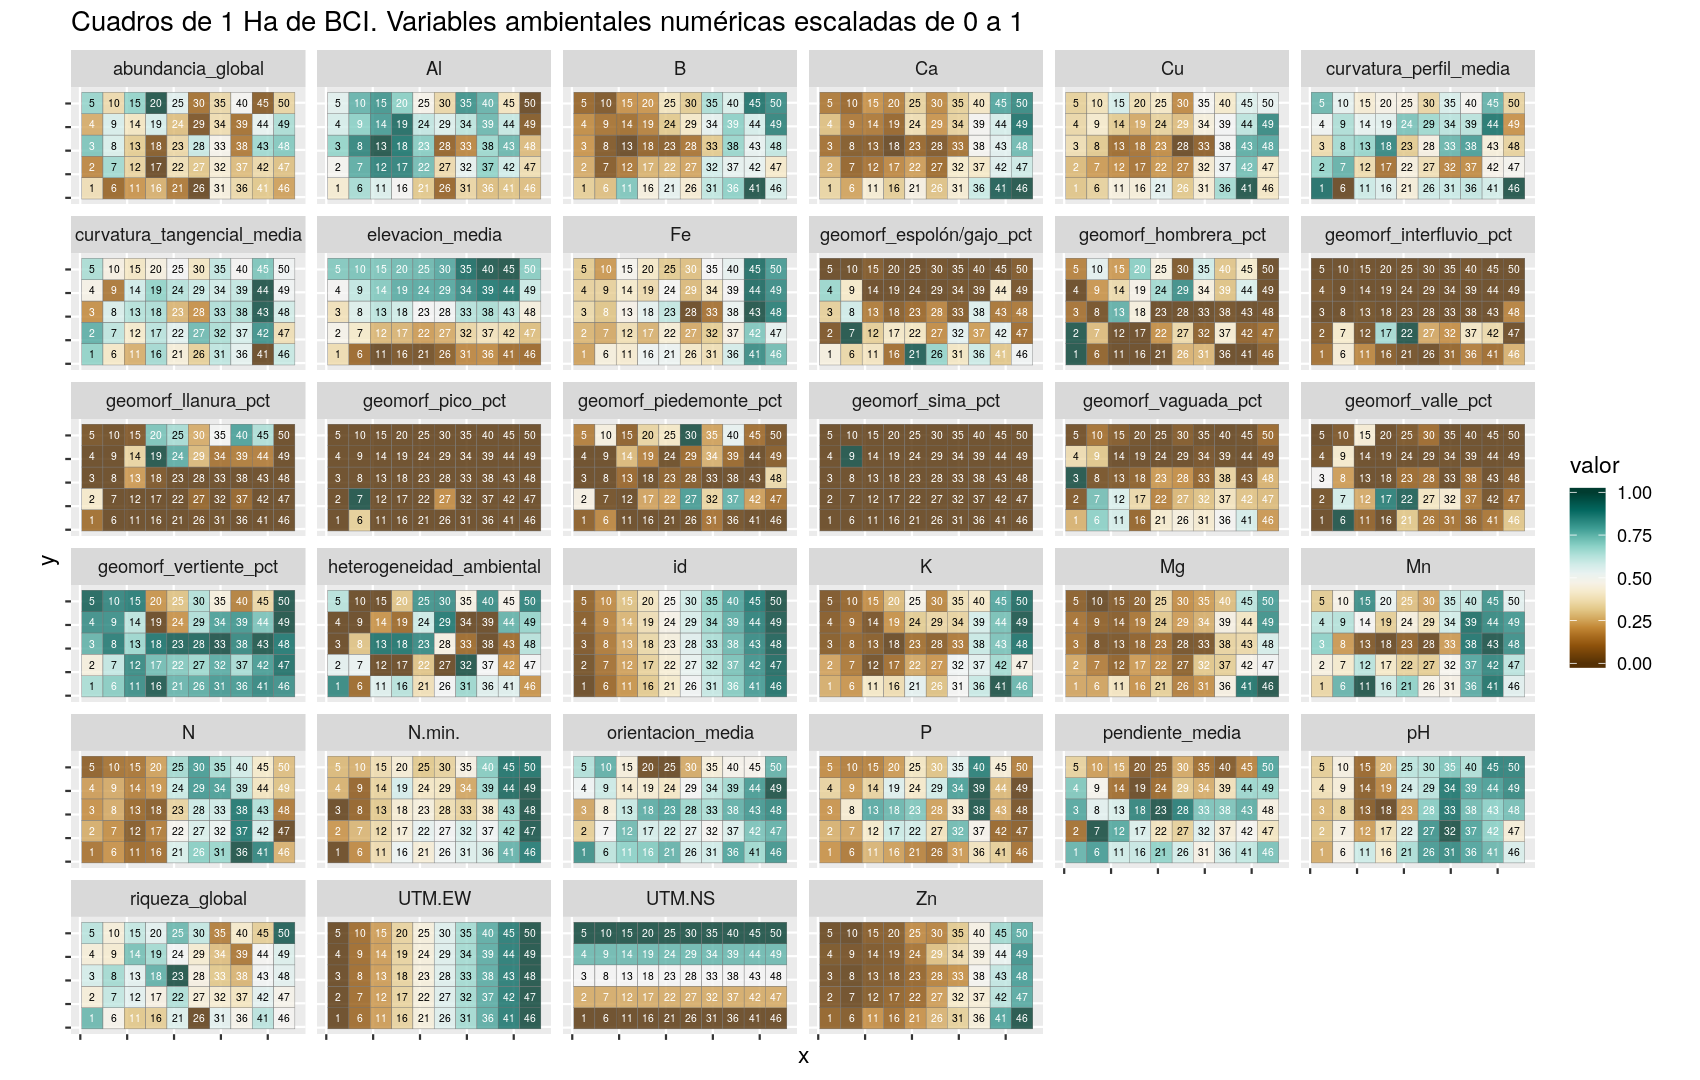
\includegraphics[width=1.00000\textwidth]{mapas_variables_ambientales_numericas.png}
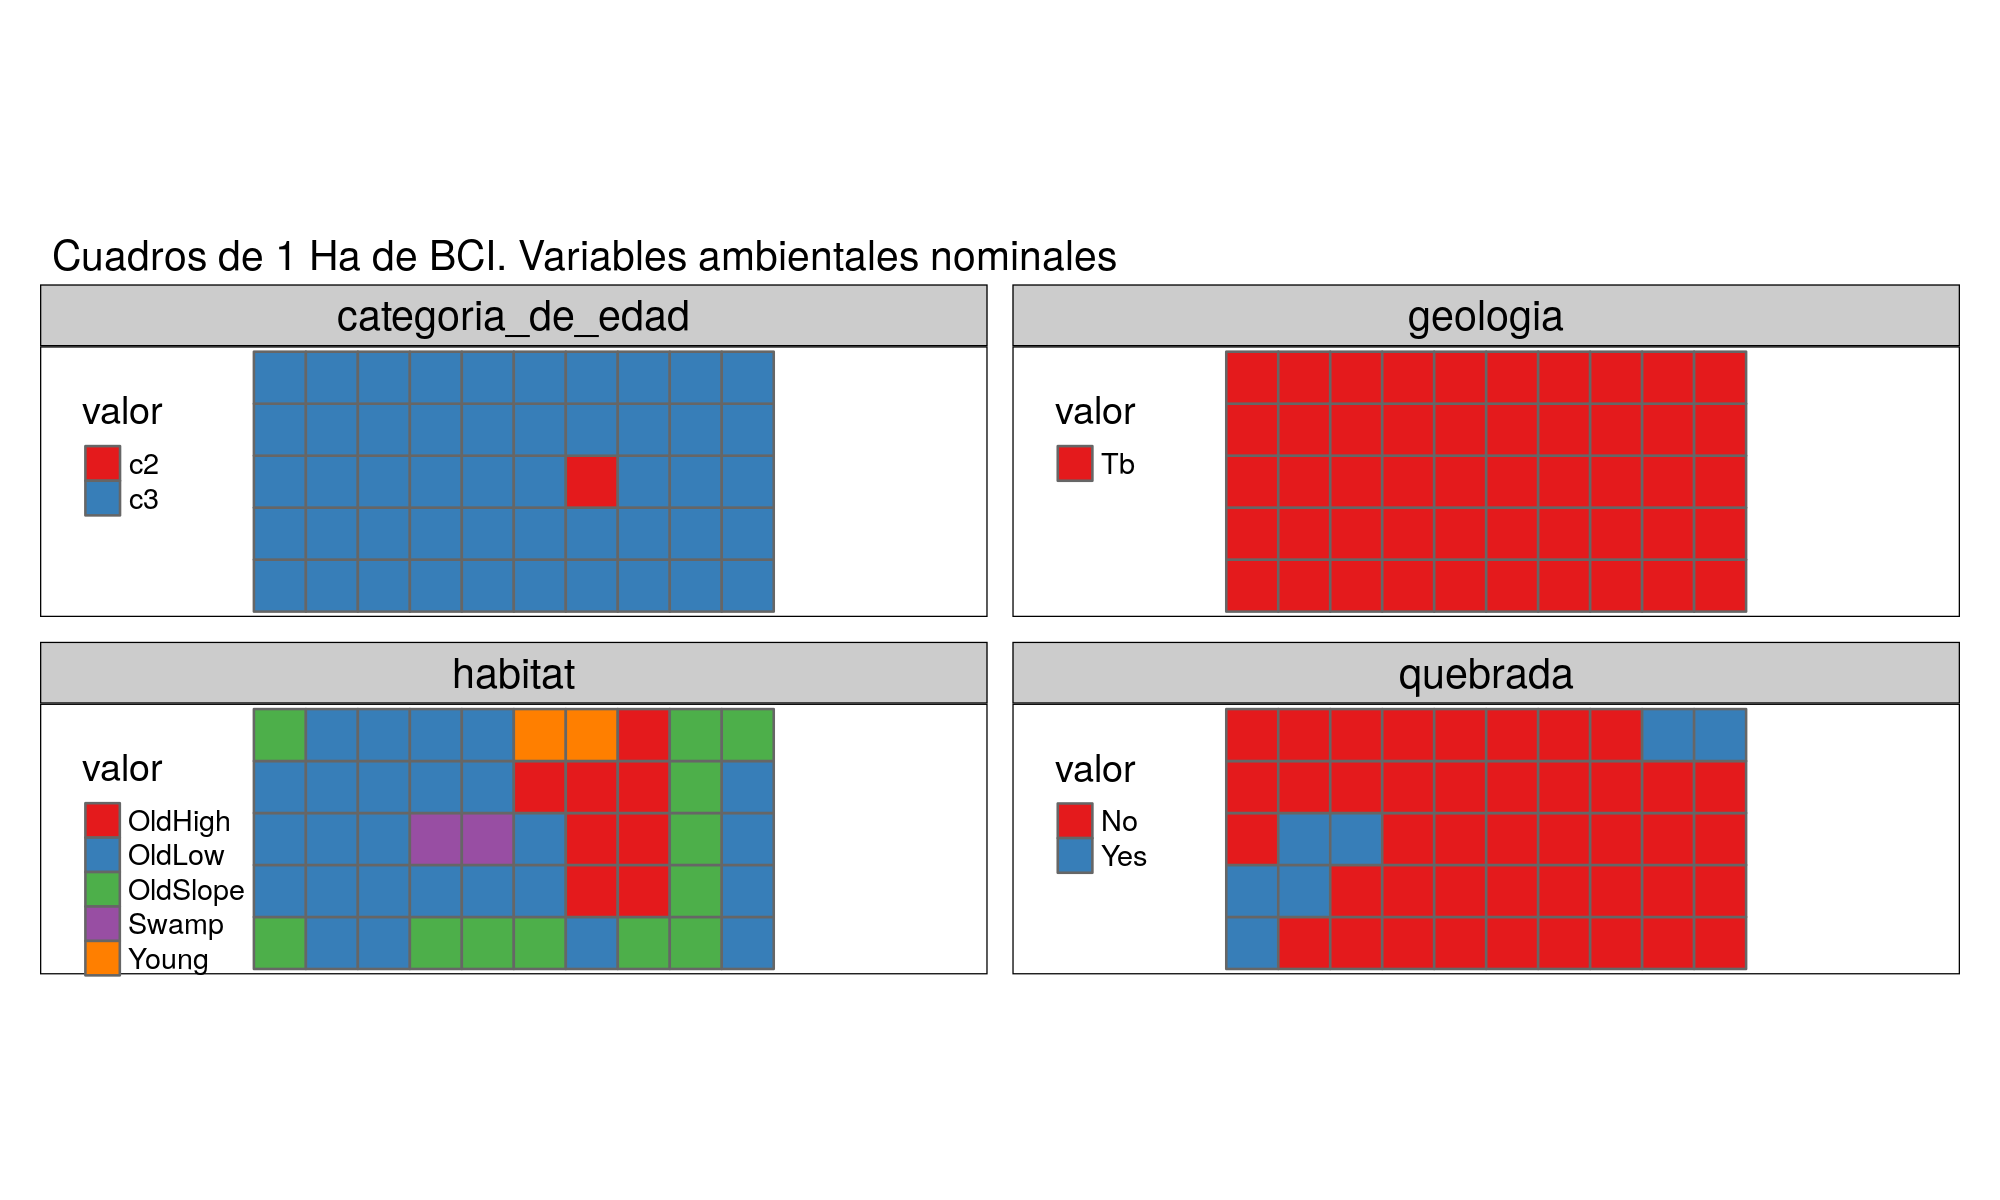
\includegraphics[width=1.00000\textwidth]{mapas_variables_ambientales_nominales_tmap.png}
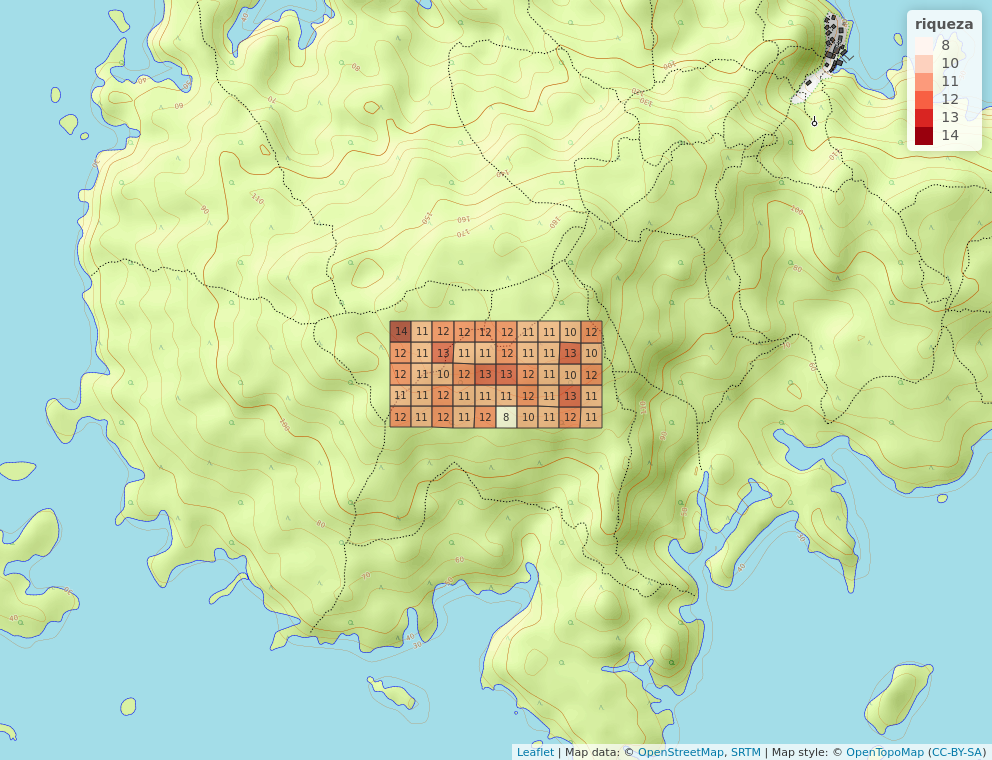
\includegraphics[width=1.00000\textwidth]{mapa_cuadros_riq_mi_familia.png}

\section{\texorpdfstring{\emph{Script}
reproducible}{Script reproducible}}\label{script-reproducible}

\ldots

\section*{Referencias}\label{referencias}
\addcontentsline{toc}{section}{Referencias}

\hypertarget{refs}{}
\hypertarget{ref-cardona2007avispas}{}
Cardona, W., De Ulloa, P. C., \& Kattan, G. (2007). Avispas no
polinizadoras asociadas a ficus andicola (moraceae) en la cordillera
central de colombia. \emph{Revista Colombiana de Entomología},
\emph{33}(2), 165--170.

\hypertarget{ref-clement2009morphological}{}
Clement, W. L., \& Weiblen, G. D. (2009). Morphological evolution in the
mulberry family (moraceae). \emph{Systematic Botany}, \emph{34}(3),
530--552.

\hypertarget{ref-fredericksenbibosi}{}
Fredericksen, T. S., Justiniano, M. J., Rumiz, D., McDonald, E., \&
Aguape, R. (n.d.). \emph{Bibosi higuerón ficus spp. moraceae}.

\hypertarget{ref-magallanesdistribucion}{}
Magallanes, A. B., Rocha, Y. R., \& Terán, F. A. (n.d.).
\emph{Distribución y abundancia de las especies arbóreas de la familia
moraceae en la reserva ecológica del mineral de nuestra señora de la
candelaria, cosalá, sinaloa}.

\hypertarget{ref-piedra2006genero}{}
Piedra-Malagón, E. M., Ramírez Rodríguez, R., \& Ibarra -Manríquez, G.
(2006). El género ficus (moraceae) en el estado de morelos, méxico.
\emph{Acta Botánica Mexicana}, (75), 45--75.

\hypertarget{ref-simmonds2002parametros}{}
Simmonds, J. A., Gómez, J. A., \& Villalaz, J. (2002). Parametros
fisico-quimicos y biologicos en aguas circundantes al canal de panama.
\emph{Tecnociencia}, \emph{4}(1), 47--69.

\hypertarget{ref-van2010biodiversidad}{}
Van Devender, T. R., Felger, R. S., Fishbein, M., Molina-Freaner, F. E.,
Sánchez-Escalante, J. J., Reina-Guerrero, A., \& others. (2010).
Biodiversidad de las plantas vasculares. \emph{Diversidad Biológica de
Sonora. Universidad Nacional Autónoma de México. México, DF, México},
229--261.

\hypertarget{ref-williams2002patrones}{}
Williams-Linera, G., \& Meave, J. (2002). Patrones fenológicos.
\emph{Ecología Y Conservación de Bosques Neotropicales, RM Guariguata Y
GH Kattan (Eds .). Libro Universitario Regional, San José}, 591--624.




\newpage
\singlespacing 
\end{document}
